\chapter{Generalised Off-line Training of Spiking Neural Networks}
\label{cha:Conv}
%Paragraph One: LINK
%In the last chapter, we answered our first research question of validating the capability of real-time cognitive application built on neuromorphic platform by building an object recognition prototype running completely on hardware in an absolute spike-based fashion.
%It built up the basis for the later research that neuromorphic hardware has been capable of running large applications standing alone without a general computer.

In the last chapter, we have illustrated the promising Deep Learning research in the field of artificial neural networks~(ANNs). 
An intuitive idea of bringing these Deep Learning techniques to spiking neural networks~(SNNs) is to operate deep SNNs using the trained weights of the equivalent ANNs.
Hence SNNs can be trained by first training an equivalent ANN and then transferring the trained weights to the SNN.
We call this method `off-line', since the training does not take place on SNNs directly, but rather on ANNs instead.
This chapter proposes a generalised off-line training of SNNs to address the first research problem of the thesis: how to train SNNs on equivalent ANNs, thus to make trained SNNs as competent as ANNs in cognitive tasks. 

%Paragraph Two: FOCUS
%Now focus the reader’s attention on what this chapter is specifically going to do and why it is important. In this chapter I will examine.. I will present… I will report … This is crucial in (aim of thesis/research question) in order to….

There are two significant problems to be solved when training SNNs off-line.
First, an accurate activation function is needed to model the neural dynamics of spiking neurons.
In this chapter, we propose an activation function, 
Noisy Softplus~(NSP), which closely models the response firing activity of Leaky Integrate-and-Fire~(LIF) neurons.
The second problem is mapping the abstract numerical values of the ANN to concrete physical units in the SNN, such as current and firing rate.
Thus we introduce the parametric activation function~(PAF: $y = p \times f(x)$), to tackle this problem.
With these problems solved, SNN training can be simplified as: (1) estimate parameter $p$ for PAF according to biological configurations of LIF neurons, and (2) use PAF instead of conventional activation functions to train an equivalent ANN.
The trained weights can be transferred directly into the spiking version of the same network without further conversion.
In addition, we propose a fine tuning method as an option which helps the trained network to closer match the SNN.
Based on this generalised training method, we achieve the best SNN accuracy on the MNIST task using LIF neurons, 99.07\%, on a 6-layer spiking convolutional neural network~(ConvNet).

In this chapter, we begin by introducing existing solutions of off-line SNN training in Section~\ref{sec:intro_NSP}.
We then propose the novel activation function, NSP, and demonstrate how it fits the network dynamics composed of spiking neurons in Section~\ref{sec:response_func}.
Section~\ref{sec:genrial_SNN} illustrates the generalised SNN training method using PAFs.
In Section~\ref{sec:iconipResult} we demonstrate the training of a spiking ConvNet, and compare the proposed method to existing training algorithms.

\section{Introduction}
\label{sec:intro_NSP}

%%How to map a well trained ANN to SNN is a hot topic in this field, especially using spiking neurons of biological scale.
%
%Conversely, the offline training of an ANN, which is then mapped to an SNN, has shown near loss-less conversion and state-of-the-art classification accuracy.
%This research aims to prove that SNNs are equally capable as their non-spiking rivals of pattern recognition, and at the same time are more biologically realistic and energy-efficient.
%Jug et al.~\cite{Jug_etal_2012} first proposed the use of the Siegert function to replace the sigmoid activation function in training Restricted Boltzmann Machine (RBM).
%The Siegert units map incoming currents driven by Poisson spike trains to the response firing rate of a Leaky Integrate-and-Fire (LIF) neuron.
%The ratio of the spiking rate to its maximum is equivalent to the output of a sigmoid neuron.
%A spiking Deep Belief Network (DBN)~\cite{Stromatias2015scalable} of four layers of RBMs was implemented on neuromorphic hardware, SpiNNaker~\cite{furber2014spinnaker}, to recognise hand written digits in real time.
%
%However, cortical neurons seldom saturate their firing rate as sigmoid neurons.
%Thus ReLU were proposed to replace sigmoid neurons and surpassed the performance of other popular activation units thanks to their advantage of sparsity~\cite{glorot2011deep} and robustness towards the vanishing gradient problem. % which will be described in Section~\ref{sec:activation}.
%%TODO Chapter2 about relu and vanishing gradient problem.
%%	~\cite{dugas2001incorporating}.
%%trained with noisy input, the 4-layered spiking autoencoder reached 98.37\% accuracy on MNIST. 
%Recent developments on ANN-trained SNN models has focused on using ReLU units and converting trained weights to fit in SNNs.
%Better performance~\cite{cao2015spiking,diehl2015fast} than Siegert-trained RBM has been demonstrated in Spiking ConvNets, but this method is designed for simple integrate and fire (IF) neurons without leakage and requires extra step for converting ANN-trained weights for SNN use.
%The training used only ReLUs and zero bias to avoid negative outputs, and applied a deep learning technique, dropout~\cite{srivastava2014dropout}, to increase the classification accuracy.
%Normalising the trained weights for use on an SNN employing IF neurons only was relatively straightforward and maintained classification accuracy.
%This work was extended to a Recursive Neural Network (RNN)~\cite{diehl2016conversion} and run on the TrueNorth~\cite{merolla2014million} neuromorphic hardware platform.
%
%Except for the popular, simplified version of ReLU, $max(0,\sum w x)$, the other implementation of $\log(1+e^x)$, `Softplus', is more biologically realistic.
%Recent work~\cite{hunsberger2015spiking} proposed the Soft LIF response function for training SNNs, which is equivalent to Softplus activation of ANNs.
%	
%\section{Modelling The Activation Function}
%\label{sec:af_model}
%We have introduced the existing work of modelling the response firing activity of LIF neurons using Siegert~\cite{Jug_etal_2012} function.
%It suggested an approach to modelling activation functions for spiking neurons whose input is a synaptic current generated by spike arrivals and whose output is the firing rate of a sequence of spikes.
%This section will start from the neural science background to demonstrate those physical quantities used in the Siegert formula.
%Then we will compare and show the difference between analytical estimation and practical simulations of spiking neurons.
%Consequently, we propose the new activation function, Noisy Softplus, to replace Siegert function for modelling the practical spiking activities of LIF neurons.

	
	
%	Advances in computing power and deep learning have benefited computers with a rapidly growing performance in cognitive tasks, such as recognising objects~\cite{deng2009imagenet} and playing GO~\cite{silver2016mastering}. 
%	These tasks were once dominated by human intelligence and solved by biological neurons in the brain.
%	However, humans and many other animals still win against computers in practical tasks and outperform in the terms of size and energy by several orders of magnitude.
%	For instance, AlphaGO~\cite{silver2016mastering} consumed 1~MW of power on its 1920 CPUs and 280 GPUs when playing the game with one of the best human players whose brain merely consumed about 20~W.
%	
%	Although we are still far from understanding the brain thoroughly, it is believed that the performance gap between computation in the biological nervous system and in a computer lies in the fundamental computing units and how they compute.
%	Computers employ Boolean logic and deterministic digital operations based usually on synchronous clocks while nervous systems employ parallel-distributed, event-driven, stochastically unreliable components~\cite{indiveri2009artificial}, neurons.
%	The impressive disparities in cognitive capabilities and energy consumption drives the research into biologically-plausible spiking neurons and brain inspired computers, known as neuromorphic engineering~\cite{furber2016large}.
	
	We have specified the differences of a conventional artificial neuron and a spiking neuron in Section~\ref{sec:spike}: regular artificial neuron comprises a weighted summation of input data, $\sum x_i w_i$, and an activation function, $f$, applied on the sum.
%	Usually, a bias is included in the weighted summation which can be seen as an extra input $x_b = 1$ with its weight set to $b$.
%	However, in this thesis we exclude biases for both artificial and spiking neurons to simplify neural models and to reduce the number of parameters.
	However the inputs of a spiking neuron (Figure~\ref{Fig:compare_as4}) are spike trains, which generates current influx through neural synapses (connections).
	A single spike creates a current pulse with an amplitude of $w$, which is defined as the synaptic efficacy, and the current then decays exponentially with a decaying rate determined by the synaptic time constant, $\tau_{\textit{\textrm{syn}}}$.
	The current pulses then consequently produce post-synaptic potentials~(PSPs) on the neuron driving its membrane potential change over time, and trigger spikes as outcomes when the neuron's membrane potential reaches some threshold.
	The dynamics of the current influxes, PSPs, membrane potentials, and spike trains are all time dependent, while neurons of ANNs only cope with abstract numerical values representing spiking rate, without timing information.
%	It is the stochasticity, in contrast to the continuously differentiable functions used by ANNs, that is intrinsic to the event-based spiking process, making network training difficult.
	Therefore, these fundamental differences in input/output representation and neural computation raise the main research problem of how to operate and train biologically-plausible SNNs to make them as competent as ANNs in cognitive tasks.
	In this chapter, we focus on the specific research problem of off-line SNN training where SNNs are trained on equivalent ANNs and then the trained weights are transferred to the SNNs.
	
	\begin{figure}[tb!]
		\centering
%		\begin{subfigure}[t]{0.38\textwidth}
%			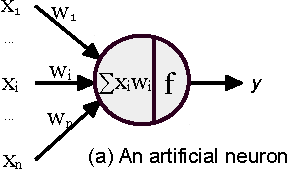
\includegraphics[width=\textwidth]{pics_iconip/neuron_ann.pdf}
%			%			\caption{Current sampled at $dt$=1~ms.}
%		\end{subfigure}~\\
		\begin{subfigure}[t]{0.85\textwidth}
			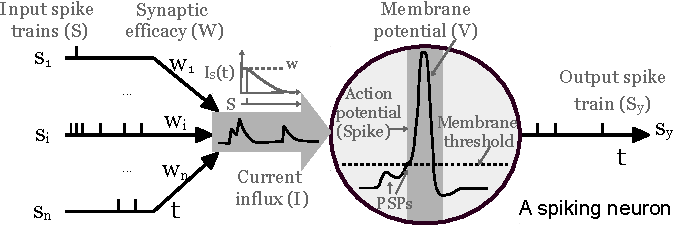
\includegraphics[width=\textwidth]{pics_iconip/neuron_snn.pdf}
			%			\caption{Current sampled at $dt$=10~ms.}
		\end{subfigure}
		\caption{A spiking neuron. Spike trains flow into a spiking neuron as current influx, trigger linearly summed PSPs through synapses with different synaptic efficacy \textbf{w}, and the post-synaptic neuron generates output spikes when the membrane potential reaches some threshold.}
		\label{Fig:compare_as4}
	\end{figure}
	
%	An intuitive idea is to train SNNs on an equivalent ANN and then transfer the trained weights to the SNN.
	
	Jug et al.~\cite{Jug_etal_2012} first proposed the use of the Siegert formula~\cite{siegert1951first} as the activation function in training Deep Belief Networks, which maps incoming currents driven by Poisson spike trains to the response firing rate of an LIF neuron.
	The variables of the activation function are in physical units, thus the trained weights can be transferred directly into SNNs.
	%Jug et al\cite{Jug_etal_2012} first proposed the use of the Siegert function to replace the sigmoid activation function in training Restricted Boltzmann Machines (RBMs).
	%The Siegert units map incoming currents driven by Poisson spike trains to the response firing rate of an LIF neuron.
	%The ratio of the spiking rate to its maximum is equivalent to the output of a sigmoid neuron.
	%A spiking Deep Belief Network (DBN)~\cite{Stromatias2015scalable} of four layers of RBMs was implemented on neuromorphic hardware, SpiNNaker~\cite{furber2014spinnaker}, to recognise hand written digits in real time.
	However, the Siegert formula is inaccurate as it models the current noise as white~\cite{liu2016noisy}, $\tau_{\textit{\textrm{syn}}} \to 0$, but it is not feasible in practice.
	%	taking no notice of the coloured noise generated by the synaptic time constant $\tau_{\textit{\textrm{syn}}}$ of spike arrivals, since the current noise is only a white noise when $\tau_{\textit{\textrm{syn}}} \to 0$~.
	Moreover, the high complexity of the Siegert function and the computation of its derivative to obtain the error gradient cause much longer training time, thus consuming more energy, when compared to regular ANN activation functions, such as Sigmoid.
	%Additionally, neurons have to fire at high frequency (higher than half of the maximum firing rate) to represent the activation of a sigmoid unit; thus the network activity results in high power dissipation.
	%Hence researchers turned to abstract activation functions to model the response activity of spiking neurons to simplify the computation. %and at the same time improve the model accuracy of the activation function.
	%	A similar activation function of Soft LIF~\cite{hunsberger2015spiking} was introduced to simplify the computation complexity.
	We will illustrate these problems in detail in Section~\ref{sec:response_func}. %{sec:siergert} and~\ref{subsec:practice}.
	
	A softened version of the response function of LIF neurons is proposed~\cite{hunsberger2015spiking} and is less computationally expensive than the Siegert function.
	However, the model ignored the dynamic noise change introduced by input spikes, assuming static noise level of the current influx.
	Therefore the training required additional noise on the response firing rate and on the training data, thus included hyper-parameters in the model.
	%	What's more, the activation function compromised the modelling accuracy for computational simplicity.
	
	
	Although both the LIF response functions take and output variables in physical units such that the trained weights can be directly used in SNNs, they struggle in poor modelling accuracy and high computation complexity.
	Besides, the disadvantage of response functions employing physical units is that they lose the numerical abstraction of firing rates in ANNs, thus they can be only used for training SNNs, meanwhile other widely-used activation functions of ANNs cannot be transformed to fit in SNN training. 
	Therefore, the first problem of off-line SNN training is the accurate modelling of the neural response activity of LIF neurons using abstract activation functions, in the hope of (1) increasing the performance of SNN training, (2) reducing the computation complexity and (3) generalising off-line SNN training to the way of training ANNs.
	We call activation functions `abstract' referring to the ones without physical units which are used in the ANNs, and select them for LIF modelling due to their simplicity and generalised use for training ANNs.
	Thus we propose the activation function, NSP~\cite{liu2016noisy}, in Section~\ref{sec:NSP} to address this problem.
%	Thus, NSP~\cite{liu2016noisy} (Section~\ref{sec:NSP}), we proposed closely match the response activity of LIF neurons by including current noise as the second factor in the activation function and taking account of coloured noise driven by $\tau_{\textit{\textrm{syn}}}$.
	
	
	
	Then the second problem is to map the abstract activation functions to physical units: current in nA and firing rates in Hz, hence the trained weights of ANNs with such mapped activation functions can be used in SNNs without conversion.
	%Better learning performance has been reported using ReLU, so modelling ReLU-like activation function for spiking neurons is needed.  
	%Based on the fact that cortical neurons seldom saturate their firing rate as sigmoid neurons,ReLU~\cite{glorot2011deep} were proposed to replace sigmoid neurons and surpassed the performance of other popular activation units.
	%trained with noisy input, the 4-layered spiking autoencoder reached 98.37\% accuracy on MNIST. 
	Instead of directly solving this problem, an alternative way is to train an ANN with abstract activation functions and then convert the trained weights to fit in SNNs.
	Researchers~\cite{cao2015spiking,diehl2015fast} successfully applied this method on less biologically-realistic and simplified integrate-and-fire (IF) neurons.
	Normalising the Rectified Linear Units~(ReLU)-trained weights for use on simplified IF neurons was relatively straightforward, so this method sets the state-of-the-art performance.
	However, this chapter (in Section~\ref{sec:genrial_SNN}) aims to address the second problem of mapping abstract activation functions to the response firing activity of biologically-plausible LIF neurons, thus to complete a formalised SNN training mechanism and to generalise the method to commonly-used simple activation functions, such as ReLU.
\section{Modelling the Response Function}
	\label{sec:response_func}
	\subsection{Biological Background}
	\label{sec:siergert}
	%As discussed above, most of the top scored networks map the ReLUs in ANN to the equivalent spiking version of IF neurons.
	%This research proposes a new activation function, Noisy Softplus, which is inspired by neuroscience observations of LIF neurons.
	The LIF neuron model follows the following membrane potential dynamics:
	\begin{equation}
	\tau_m \frac{\D V}{\D t}=V_{rest} - V + R_{m} I(t) ~.
	\label{equ:LIF_V}
	\end{equation}
	The membrane potential $V$ changes in response to the input current $I$, starting at the resting membrane potential $V_{rest}$, where the membrane time constant is $\tau_m = R_mC_m$, $R_m$ is the membrane resistance and $C_m$ is the membrane capacitance.
	The central idea in converting spiking neurons to activation units lies in the response function of a neuron model.
	Given a constant current injection $I$, the response function, i.e. firing rate, of the LIF neuron is:
	\begin{equation}
	\lambda_\mathit{out}=
	\left [ t_\mathit{ref}-\tau_m\log \left ( 1-\frac{V_{th}-V_\mathit{rest}}{IR_m}  \right )\right ]^{-1}, \textrm{~when~} IR_m>V_{th}-V_{rest},
	\label{equ:consI}
	\end{equation}
	otherwise the membrane potential cannot reach the threshold $V_{th}$ and the output firing rate is zero. 
	The absolute refractory period $t_\mathit{ref}$ is included, during which period synaptic inputs are ignored.
	
	%TODO very important part
	However, in practice, a noisy current generated by the random arrival of spikes, rather than a constant current, flows into the neurons.
	%White noise
	The noisy current is typically treated as a sum of a deterministic constant term, $I_{const}$, and a white noise term, $I_{noise}$.
	Thus the value of the current is Gaussian distributed with $m_I$ mean and ${s_I}^2$ variance.
	The white noise is a stochastic process $\xi(t)$ with mean 0 and variance 1, which is delta-correlated, i.e., the process is uncorrelated in time so that a value $\xi(t)$ at time $t$ is totally independent on the value at any other time $t'$.
	Therefore, the noisy current can be seen as:
	\begin{equation}
	I(t) = I_{const}(t)+I_{noise}(t) = m_I + s_I\xi(t)~~,
	\label{equ:noisyI}
	\end{equation}
	and accordingly, Equation~\ref{equ:LIF_V} becomes:
	\begin{equation}
	\frac{\D V}{\D t}=\frac{V_{rest} - V}{\tau_m } + \frac{m_I}{C_m} + \frac{s_I\xi(t)}{C_m}~~.
	\label{equ:LIF_V2}
	\end{equation}
	
	We then multiply the both sides of Equation~\ref{equ:LIF_V2} by a short time step $\D t$, the stochastic differential equation of the membrane potential is: % satisfies an Ornstein-Uhlenbeck process:
	\begin{equation}
	\begin{aligned}
	\D V&= \frac{V_{rest} - V}{\tau_m }\D t + \frac{m_I}{C_m} \D t + \frac{s_I}{C_m}  \D W_t \\
	&=\frac{V_{rest} - V}{\tau_m }\D t + \frac{m_I}{C_m} \D t + \frac{s_I \sqrt{\D t}}{C_m} \xi(t)  \\
	&=\frac{V_{rest} - V}{\tau_m }\D t + \mu \D t + \sigma \xi(t) ~~. 
	\end{aligned}
	\end{equation}	
	The last term $\D W_t$ is a Wiener process, that $W_{t +\D t} - W_{t}$ obeys Gaussian distribution with mean 0 and variance $\D t$.
	The instantaneous mean $\mu$ and variance $\sigma^2$ of the change in membrane potential characterise the statistics of $V$ in a short time range, and they can be derived from the statistics of the noisy current:
	\begin{equation}
	\mu =\dfrac{m_I}{C_m}, ~~~~~ \sigma = \dfrac{s_I \sqrt{\D t}}{C_m}~.
	\end{equation}
%	A continuous-time stochastic process W(t) for t>=0 with W(0)=0 and such that the increment W(t)-W(s) is Gaussian with mean 0 and variance t-s for any 0<=s<t, and increments for nonoverlapping time intervals are independent. Brownian motion (i.e., random walk with random step sizes) is the most common example of a Wiener process.
%http://mathworld.wolfram.com/WienerProcess.html
%http://neuronaldynamics.epfl.ch/online/Ch1.S3.html about V tradractory need to write in Chapter 2.	
	The response function~\cite{rauch2003neocortical,la2008response} of the LIF neuron to a noisy current, also known as Siegert formula, is driven by the $\mu$ and $\sigma$:
	\begin{equation}
	\lambda_\mathit{out}=
	\left [ t_\mathit{ref}+\tau_m \int_{\frac{V_\mathit{rest}-\mu \tau_m }{\sigma \sqrt{\tau_m}}}^{\frac{V_{th}-\mu \tau_m }{\sigma \sqrt{\tau_m}}} \sqrt{\pi} \exp(u^{2}) (1+erf(u)) \D u \right ]^{-1} ~,
	\label{equ:siegert}
	\end{equation}
	

	
	\begin{figure}[bt]
		\centering
		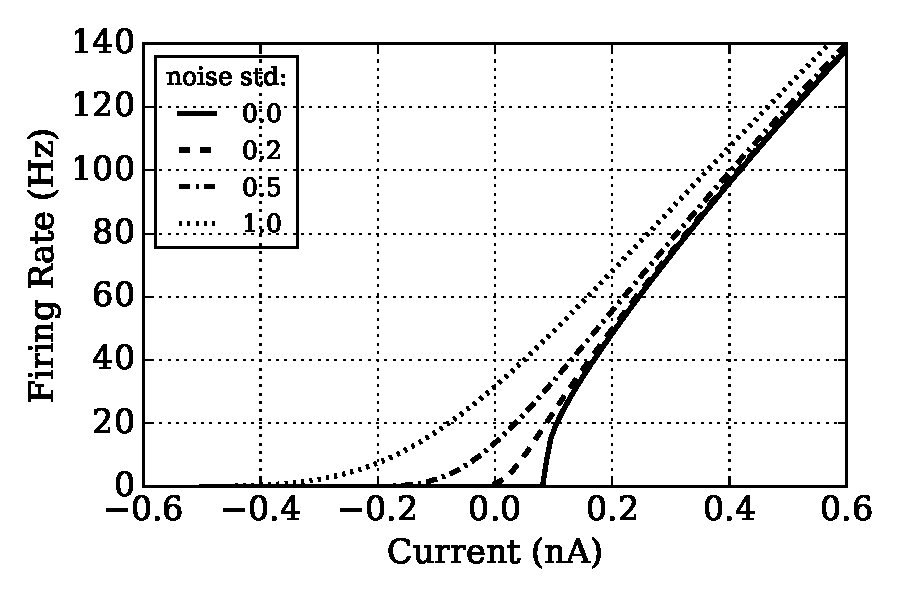
\includegraphics[width=0.7\textwidth]{pics_iconip/1.pdf}
		\caption{Response function of the LIF neuron with noisy input currents with different standard deviations.}
		\label{Fig:physics}
	\end{figure}
	
	Figure~\ref{Fig:physics} shows the response curves (Equation~\ref{equ:siegert}) of a LIF neuron driven by noisy currents with Gaussian noise of $m_I$ mean and $s_I$ standard deviation.
	The parameters of the LIF neuron are all biologically valid (see the listed values in Table~\ref{tbl:pynnConfig}), and the same parameters are used throughout this chapter.
	The solid (zero noise) line in Figure~\ref{Fig:physics} illustrates the response function of such an LIF neuron injected with constant current, which inspired the proposal of ReLUs.
	As noise increases, the level of firing rates also rises, and the Softplus activation function approximates the response firing activity driven by current with Gaussian white noise added.
	Softplus units only represent a single level of noise that, for example, the dotted line in Figure~\ref{Fig:physics} is drawn when $s_I=1$.
	
		\begin{table}[bt]
			\centering
			\caption{\label{tbl:pynnConfig}Parameter setting for the current-based LIF neurons using PyNN.}
			\bgroup
			\def\arraystretch{1.4}
			\begin{tabular}{c c c}
				%\hline
				Parameters & Values & Units \\
				\hline
				cm & 0.25 & nF	\\
				%\hline
				tau\_m & 20.0 & ms\\
				%\hline
				tau\_refrac & 1.0 & ms\\
				%					%\hline
				%					tau\_syn\_E & 5.0 & ms\\
				%					%  %\hline
				%					tau\_syn\_I & 5.0 & ms\\
				%  %\hline
				v\_reset & -65.0 & mV\\
				%\hline
				v\_rest & -65.0 & mV\\
				%\hline
				v\_thresh & -50.0 & mV\\
				%\hline
				i\_offset & 0.1 & nA\\
				\hline
				%			Parameters & cm & tau\_m & tau\_refrac & tau\_syn\_E & tau\_syn\_I & v\_rest & v\_thresh & i\_offset \\
				%			Values & 0.25 &  20.0 & 1.0 & 5.0 & 5.0 & -65.0 & -50.0  & 0.1 \\
				%			Units & nF & ms & ms & ms & ms & mV & mV& nA\\
				%			\hline
			\end{tabular}
			\egroup
		\end{table}
	

	


%	\subsection{Activation Function in ANN}
%	\label{sec:activation}
%	Nair and Hinton~\cite{nair2010rectified} stated that ReLU preserve information about relative intensities(intensity equivarance) provided they have zero biases and are noise-free, but binary units do not.
%	This technique has dominated the best recognition performances~\textcolor{red}{ref?} in deep learning.
%	Furthermore, utilising ReLU in SNNs will simplify the network structure significantly because of the zero biases.
%	Thus in this section we firstly demonstrate on how ReLU work and perform in DBN.
%	
%	The input vector in a ReLU based RBM does no longer have to be binary, so it can be a float.
%	Instead of using sigmoid transfer function, the ReLU is always positive and has no upper boundary.
%	There are three different ways to model ReLU~\ref{Fig:relu_tranf}:
%	\begin{figure}[hbt]
%		\centering
%		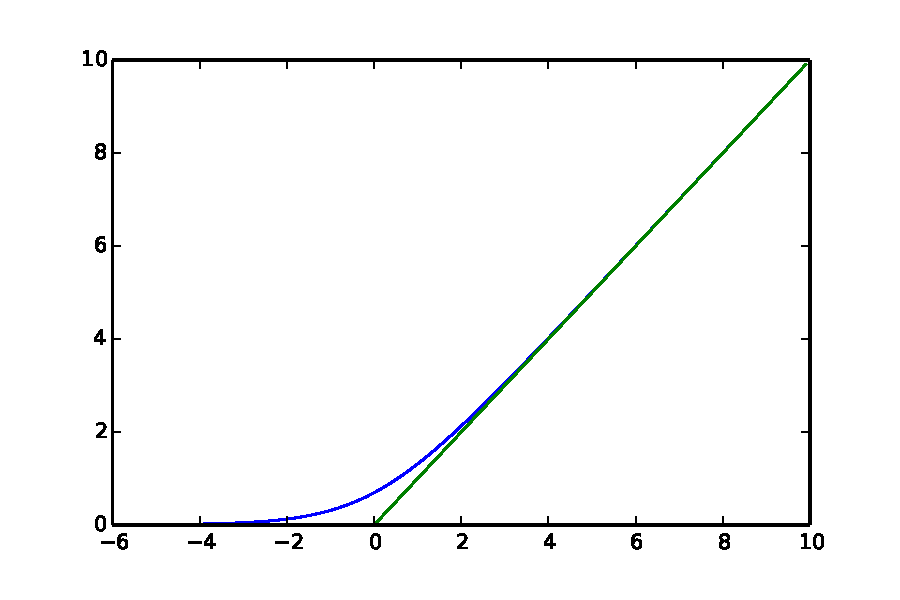
\includegraphics[width=0.7\textwidth]{pics_sdbn/relu.pdf}
%		\caption{The DBN architecture.} 
%		\label{Fig:relu_tranf}
%	\end{figure}
%	\begin{itemize}
%		\item sum of an infinite number of binary units with each having a bias less than the previous one~~\cite{nair2010rectified}.
%		This is one of the reason people believe the recognition performance exceeding since each ReLU represents infinite samples of sigmoid. 
%		\item the approximation of the previous form $\log(1+e_x)$.
%		\item the simplified version which is the most popular in deep learning $max(0,\sum w x)$.
%	\end{itemize}  
	
	
	

	
	\subsection{Mismatch of Siegert Function to Practice}
	\label{subsec:practice}
	
	
	\begin{figure}[tbp!]
		\centering
		\begin{subfigure}[t]{0.49\textwidth}
			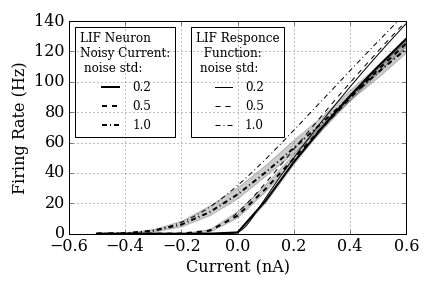
\includegraphics[width=\textwidth]{pics_iconip/2-1.png}
			\caption{Current sampled at $dt$=1~ms.}
		\end{subfigure}
		\begin{subfigure}[t]{0.49\textwidth}
			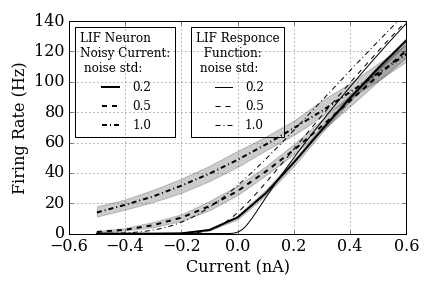
\includegraphics[width=\textwidth]{pics_iconip/2-10.png}
			\caption{Current sampled at $dt$=10~ms.}
		\end{subfigure}
		\caption{Recorded response firing rate of a LIF neuron driven by \textit{NoisyCurrentSource} sampled at every (a) 1~ms and (b) 10~ms. Averaged firing rates of 10 simulation trails are shown in bold lines, and the grey colour fills the range between the minimum to maximum of the firing rates. The analytical LIF response function, Siegert formula (Equation~\ref{equ:siegert}), is drawn in thin lines (shown in Figure~\ref{Fig:physics}) to compare with the practical simulation.}
		\label{Fig:current}
	\end{figure}
		
	\begin{figure}[tbp!]
		\centering
		\makebox[0.43\textwidth]{$dt$=1~ms} \makebox[0.43\textwidth]{$dt$=10~ms} \par
		\begin{subfigure}[t]{0.43\textwidth}
			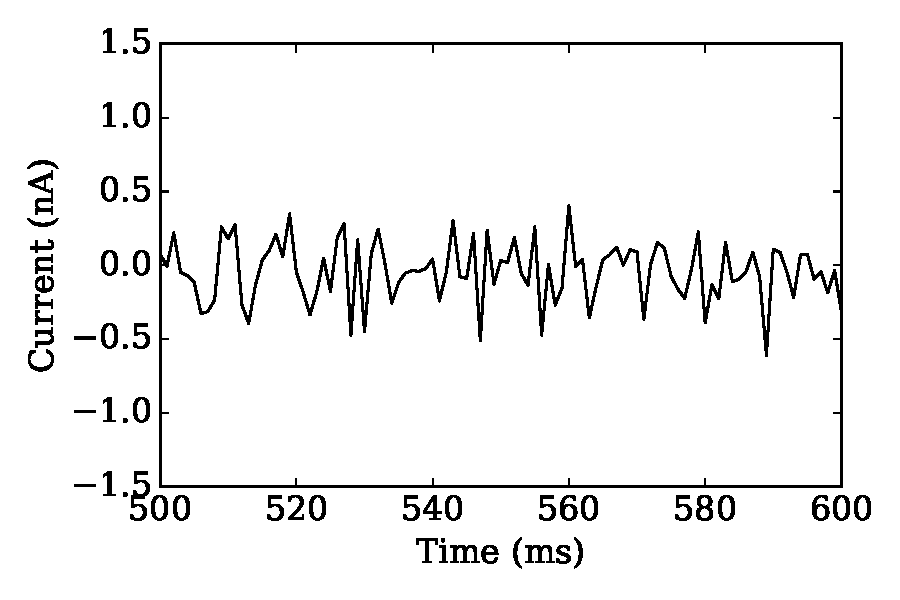
\includegraphics[width=\textwidth]{pics_iconip/curr_dt1.pdf}
			\caption{Current sampled at $dt$=1~ms.}
		\end{subfigure}
		\begin{subfigure}[t]{0.43\textwidth}
			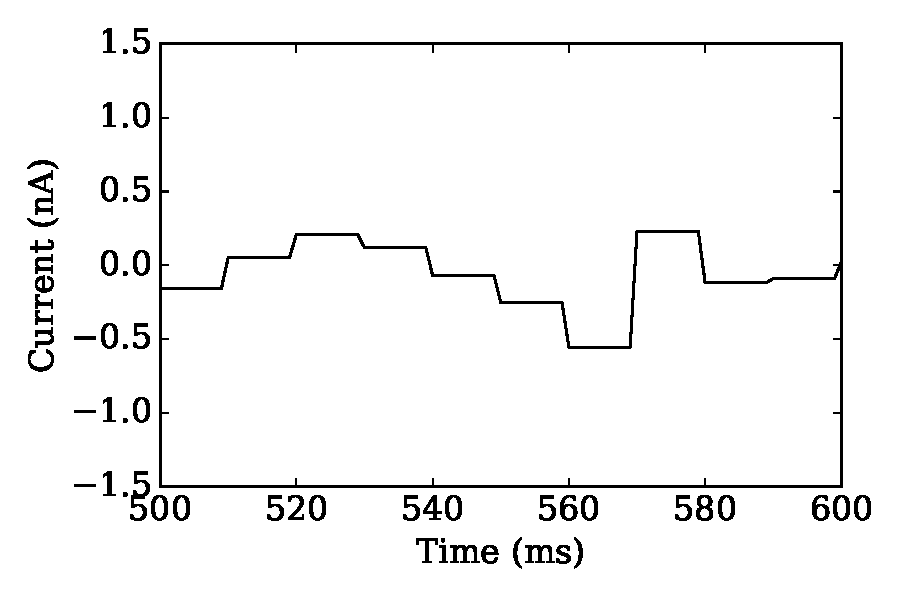
\includegraphics[width=\textwidth]{pics_iconip/curr_dt10.pdf}
			\caption{Current sampled at $dt$=10~ms.}
		\end{subfigure}\\
		\begin{subfigure}[t]{0.43\textwidth}
			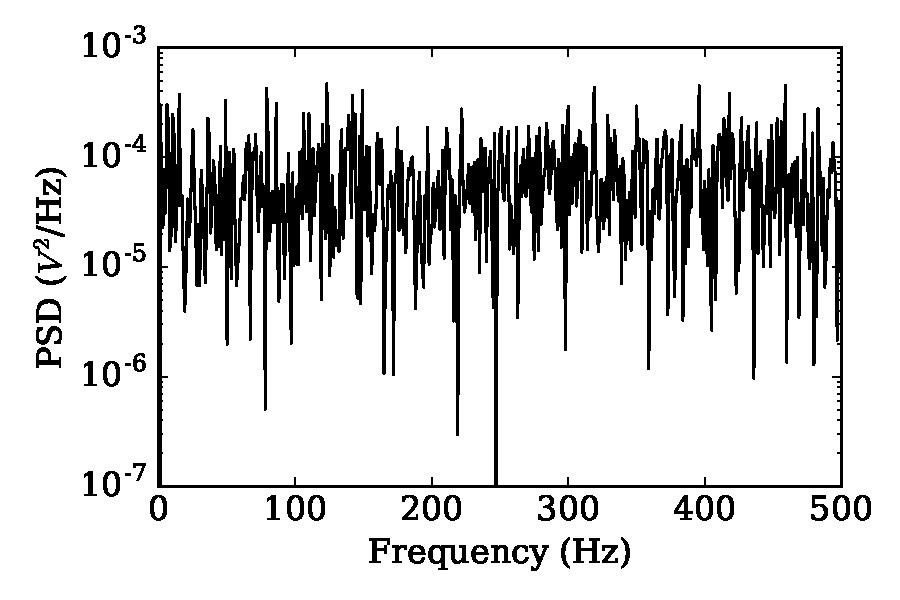
\includegraphics[width=\textwidth]{pics_iconip/psd_dt1.pdf}
			\caption{Spectrum analysis of (a).}
		\end{subfigure}
		\begin{subfigure}[t]{0.43\textwidth}
			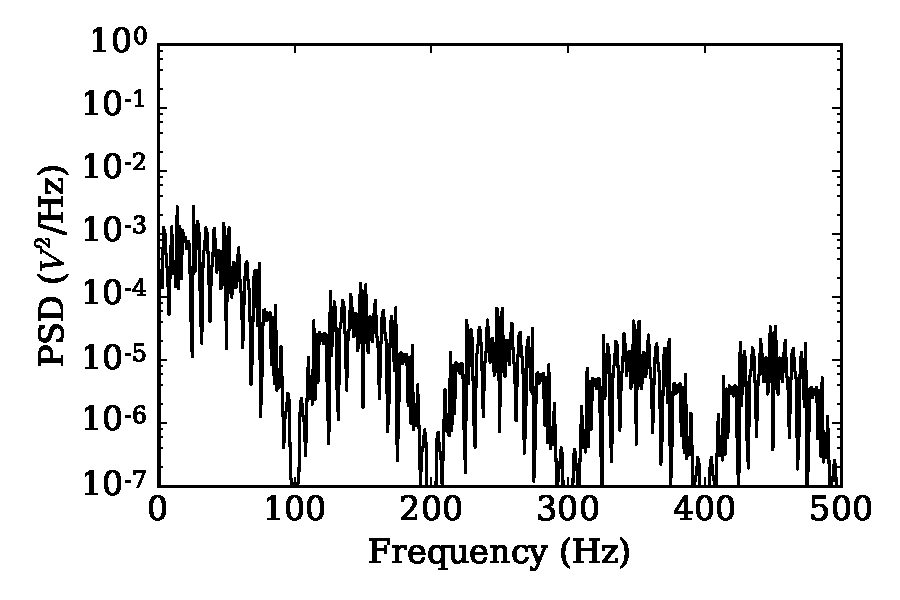
\includegraphics[width=\textwidth]{pics_iconip/psd_dt10.pdf}
			\caption{Spectrum analysis of (b).}
		\end{subfigure}\\
		\begin{subfigure}[t]{0.43\textwidth}
			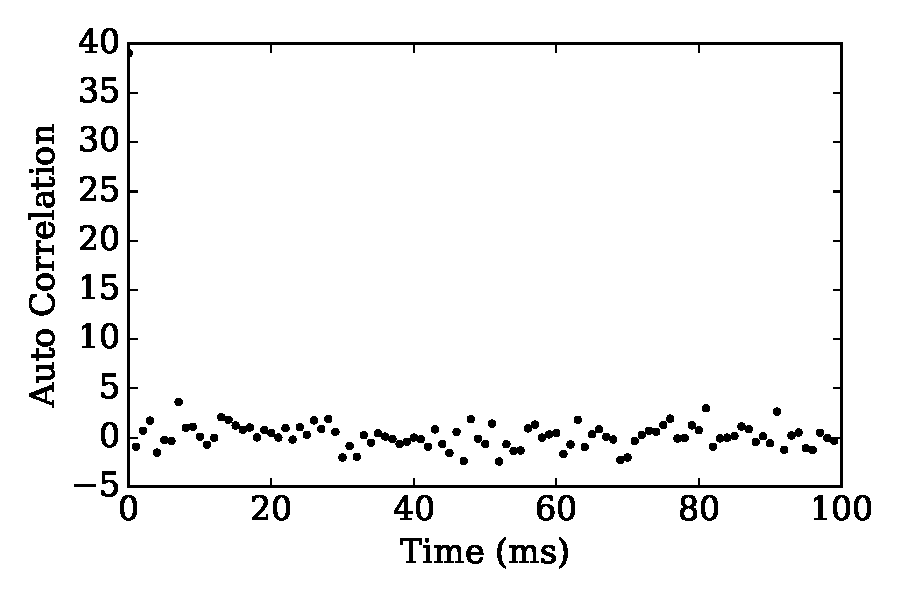
\includegraphics[width=\textwidth]{pics_iconip/autocorr_dt1.pdf}
			\caption{Autocorrelation of (a).}
		\end{subfigure}
		\begin{subfigure}[t]{0.43\textwidth}
			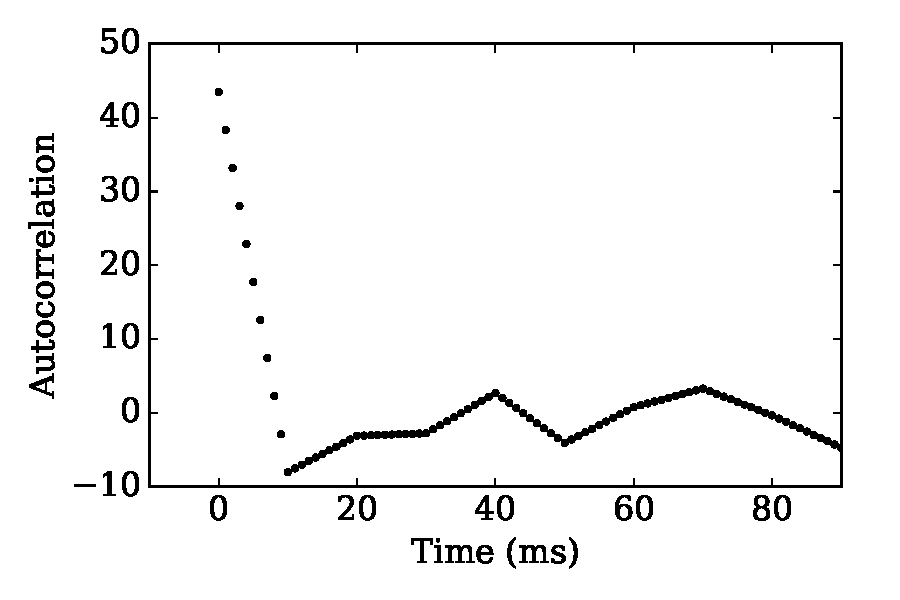
\includegraphics[width=\textwidth]{pics_iconip/autocorr_dt10.pdf}
			\caption{Autocorrelation of (b).}
		\end{subfigure}\\
		\begin{subfigure}[t]{0.43\textwidth}
			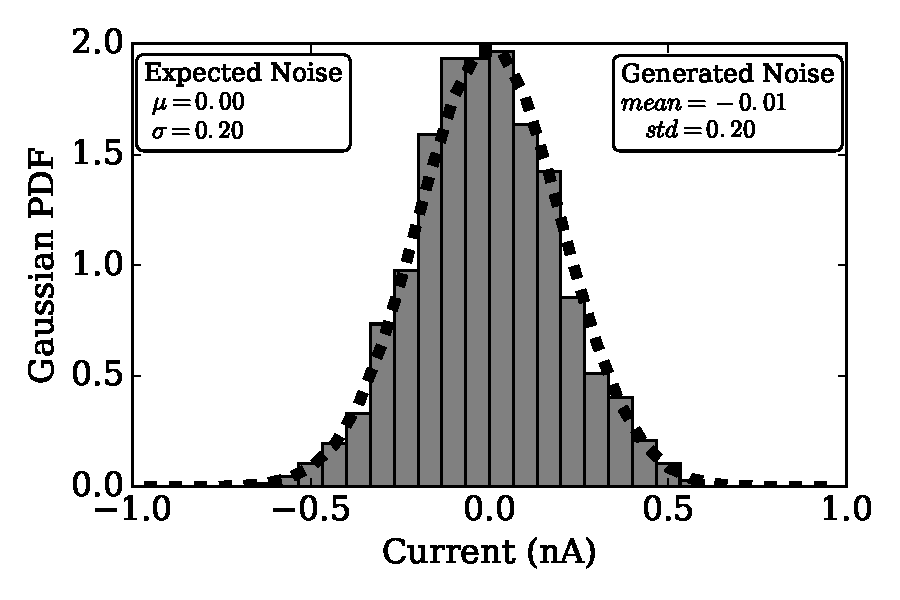
\includegraphics[width=\textwidth]{pics_iconip/distr_dt1.pdf}
			\caption{Distribution of samples of (a).}
		\end{subfigure}
		\begin{subfigure}[t]{0.43\textwidth}
			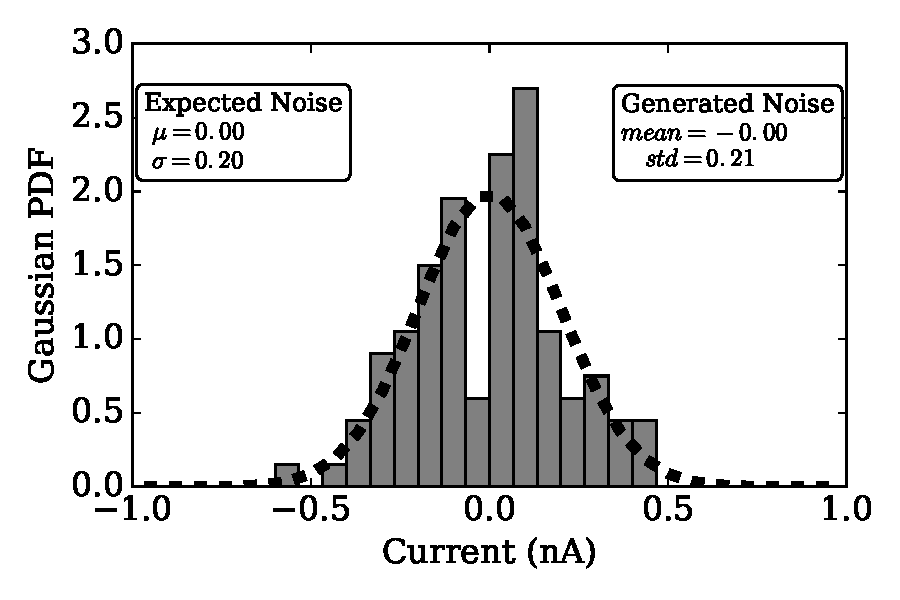
\includegraphics[width=\textwidth]{pics_iconip/distr_dt10.pdf}
			\caption{Distribution of samples of (b).}
		\end{subfigure}
		\caption{\textit{NoisyCurrentSource} samples noisy currents from Gauss distribution at every 1~ms (left) and 10~ms (right). The signals are shown in time domain in (a) and (b), and spectrum domain in (c) and (d). The autocorrelation of both current signals are shown in (e) and (f). The distribution of the discrete samples are plotted in bar chart to compare with PDF of the original Gauss distribution, shown in (g) and (h).}
		\label{Fig:lif_curr}
	\end{figure}
%\begin{figure}
%	\centering
%	\begin{subfigure}[c]{0.45\textwidth}\raggedleft
%%		\myrowlabel{Response Firing Rate}
%%		\raisebox{-.5\height}{\includegraphics[width=.9\textwidth]
%%			{pics_iconip/2-1.png}}\\
%%		\myrowlabel{Current}
%		\makebox[0.9\textwidth]{$dt$=1~ms} \par
%		\raisebox{-.5\height}{\includegraphics[width=.9\textwidth]
%			{pics_iconip/curr_dt1.pdf}}\\
%%		\myrowlabel{Spectrum Analysis}
%		\raisebox{-.5\height}{\includegraphics[width=.9\textwidth]
%			{pics_iconip/psd_dt1.pdf}}\\
%%		\myrowlabel{Autocorrelation}
%		\raisebox{-.5\height}{\includegraphics[width=.9\textwidth]
%			{pics_iconip/autocorr_dt1.pdf}}\\
%%		\myrowlabel{Distribution}
%		\raisebox{-.5\height}{\includegraphics[width=.9\textwidth]
%			{pics_iconip/distr_dt1.pdf}}
%		\caption{Current sampled at every $dt$=1~ms.}
%	\end{subfigure}%
%	\hspace{1em}
%	\begin{subfigure}[c]{0.45\textwidth}\raggedleft
%%		\raisebox{-.5\height}{\includegraphics[width=.9\textwidth]
%%			{pics_iconip/2-10.png}}\\
%		\makebox[0.9\textwidth]{$dt$=10~ms} \par
%		\raisebox{-.5\height}{\includegraphics[width=.9\textwidth]
%			{pics_iconip/curr_dt10.pdf}}\\
%		\raisebox{-.5\height}{\includegraphics[width=.9\textwidth]
%			{pics_iconip/psd_dt10.pdf}}\\
%		\raisebox{-.5\height}{\includegraphics[width=.9\textwidth]
%			{pics_iconip/autocorr_dt10.pdf}}
%		\raisebox{-.5\height}{\includegraphics[width=.9\textwidth]
%			{pics_iconip/distr_dt10.pdf}}
%		\caption{Current sampled at every $dt$=10~ms.}
%	\end{subfigure}%
%	\caption{ \textit{NoisyCurrentSource} sampled at (a) every 1~ms and (b) 10~ms. The current sources are shown in time domain and spectrum domain., so as its autocorrelation, and the distribution.}
%	\label{Fig:lif_curr}
%\end{figure}

	To verify the response function in practice, simulation tests were carried out using PyNN~\cite{davison2008pynn} to compare with the analytical results~(the Siegert function).
	The noisy current was produced by \textit{NoisyCurrentSource} in PyNN which is a constant current of $m_I$ added to a Gaussian white noise of zero mean and $s_I^2$ variance.
	The noise was drawn from the Gaussian distribution in a time resolution of $dt$.
	We chose $dt=1$~ms which is the finest resolution for common SNN simulators, and $dt=10$~ms for comparison.
	For a given pair of $m_I$ and $s_I^2$, a noisy current was injected into a current-based LIF neuron for 10~s, and the output firing rate was the average over 10 trials.
	
	The curves in Figures~\ref{Fig:current} illustrate output firing rate driven by different level of noise.
	The differences relative to the analytical results (thin lines) is due to the time resolution, $dt$, of the \textit{NoisyCurrentSource}.
	The sampled signals are shown in Figures~\ref{Fig:lif_curr}~(a) and (b).
	The discrete sampling of the noisy current introduces time step correlation to the white noise, shown in Figures~\ref{Fig:lif_curr}~(e) and (f), where the value remains the same within a time step $dt$.
	Although both current signals followed the same Gaussian distribution, see Figures~\ref{Fig:lif_curr}~(g) and (h), the current is a white noise when $dt=1$~ms, but a coloured noise, e.g. increased Power Spectral Density~(PSD) at lower frequency, when $dt=10$~ms, see Figures~\ref{Fig:lif_curr}~(c) and (d).
	Thus the Siegert formula, Equation~\ref{equ:siegert}, can only approximate the LIF response of noisy current with white noise.


%\begin{figure}
%	\centering
%	\begin{subfigure}[c]{0.45\textwidth}\raggedleft
%		\myrowlabel{Response Firing Rate}
%		\raisebox{-.5\height}{\includegraphics[width=.9\textwidth]
%			{pics_iconip/spiked_curve_1.png}}\\
%		\myrowlabel{Current}
%		\raisebox{-.5\height}{\includegraphics[width=.9\textwidth]
%			{pics_iconip/curr_tau1.pdf}}\\
%		\myrowlabel{Spectrum Analysis}
%		\raisebox{-.5\height}{\includegraphics[width=.9\textwidth]
%			{pics_iconip/psd_tau1.pdf}}\\
%		\myrowlabel{Autocorrelation}
%		\raisebox{-.5\height}{\includegraphics[width=.9\textwidth]
%			{pics_iconip/autocorr_tau1.pdf}}\\
%		\myrowlabel{Distribution}
%		\raisebox{-.5\height}{\includegraphics[width=.9\textwidth]
%			{pics_iconip/distr_tau1.pdf}}
%		\caption{$\tau_{syn}$=1~ms}
%	\end{subfigure}%
%	\hspace{1em}
%	\begin{subfigure}[c]{0.45\textwidth}\raggedleft
%		\raisebox{-.5\height}{\includegraphics[width=.9\textwidth]
%			{pics_iconip/spiked_curve_10.png}}\\
%		\raisebox{-.5\height}{\includegraphics[width=.9\textwidth]
%			{pics_iconip/curr_tau10.pdf}}\\
%		\raisebox{-.5\height}{\includegraphics[width=.9\textwidth]
%			{pics_iconip/psd_tau10.pdf}}\\
%		\raisebox{-.5\height}{\includegraphics[width=.9\textwidth]
%			{pics_iconip/autocorr_tau10.pdf}}
%		\raisebox{-.5\height}{\includegraphics[width=.9\textwidth]
%			{pics_iconip/distr_tau10.pdf}}
%		\caption{$\tau_{syn}$=10~ms}
%	\end{subfigure}%
%	\caption{Recorded response firing rate of a LIF neuron driven by synaptic current (bold lines) comparing to the noisy current source (thin lines). The synaptic current is shown in time domain and spectrum domain, so as its autocorrelation, and the distribution. (a) is tested when $\tau_{syn}$=1~ms, and (b) for $\tau_{syn}$=10~ms.}
%	\label{Fig:lif_pois}
%\end{figure}
	
	\begin{figure}[tbp!]
		\centering
		\begin{subfigure}[t]{0.49\textwidth}
			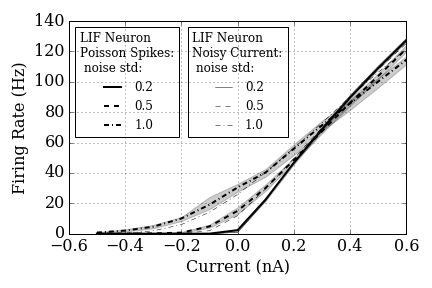
\includegraphics[width=\textwidth]{pics_iconip/spiked_curve_1.png}
			\caption{$\tau_{syn}$=1~ms.}
		\end{subfigure}
		\begin{subfigure}[t]{0.49\textwidth}
			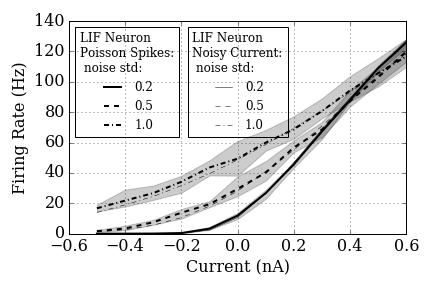
\includegraphics[width=\textwidth]{pics_iconip/spiked_curve_10.png}
			\caption{$\tau_{syn}$=10~ms.}
		\end{subfigure}
		\caption{Recorded response firing rate of a LIF neuron driven by synaptic current with two synaptic time constants: (a) $\tau_{syn}$=10~ms and (b) $\tau_{syn}$=10~ms. Averaged firing rates of 10 simulation trails are shown in bold lines, and the grey colour fills the range between the minimum to maximum of the firing rates. The firing rates recorded driven by \textit{NoisyCurrentSource}, are drawn in thin lines (shown in Figure~\ref{Fig:lif_curr}) to compare with.}
		\label{Fig:spike_curr}
	\end{figure}
	
	\begin{figure}[tbp!]
		\centering
		\makebox[0.43\textwidth]{$\tau_{syn}$=1~ms} \makebox[0.43\textwidth]{$\tau_{syn}$=10~ms} \par
		\begin{subfigure}[t]{0.43\textwidth}
			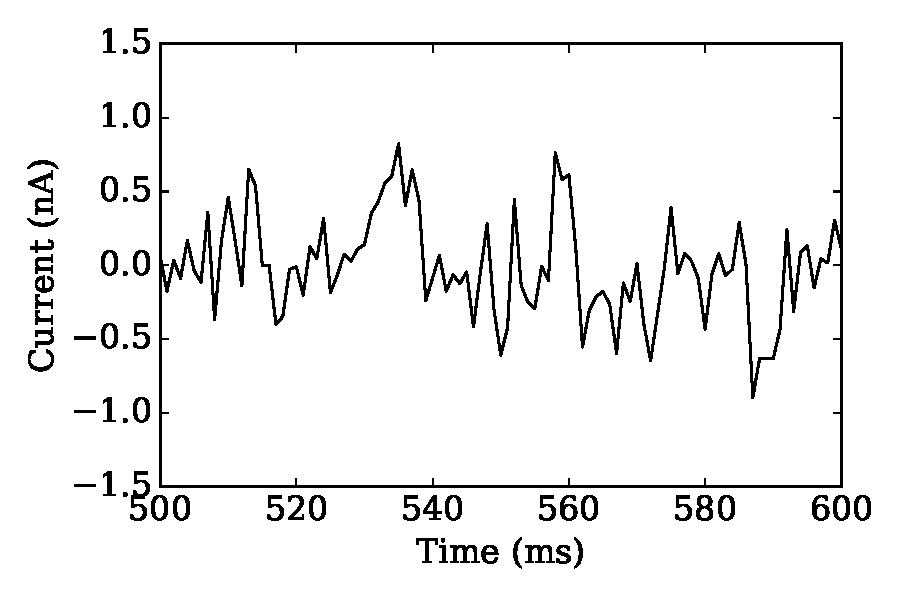
\includegraphics[width=\textwidth]{pics_iconip/curr_tau1.pdf}
			\caption{Current sampled at $dt$=1~ms.}
		\end{subfigure}
		\begin{subfigure}[t]{0.43\textwidth}
			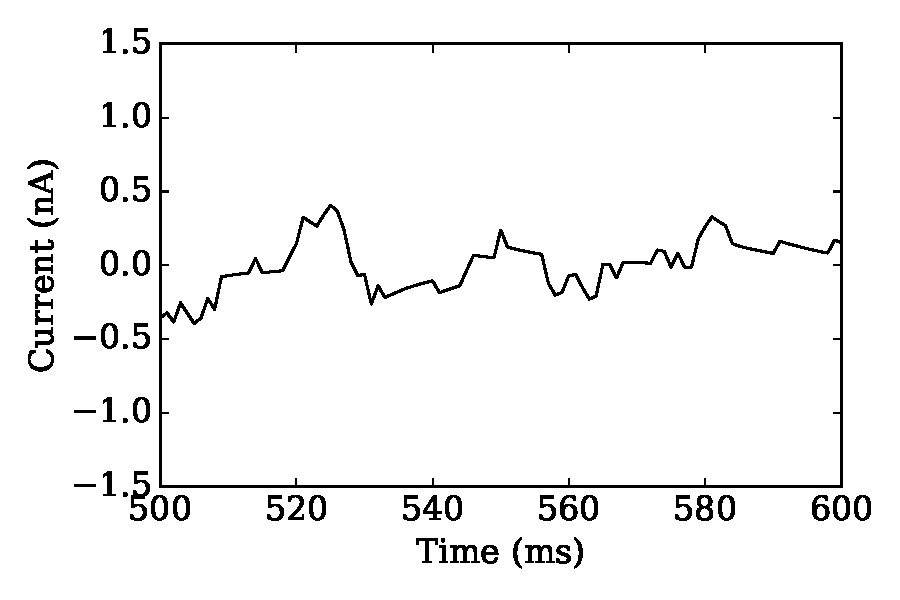
\includegraphics[width=\textwidth]{pics_iconip/curr_tau10.pdf}
			\caption{Current sampled at $dt$=10~ms.}
		\end{subfigure}\\
		\begin{subfigure}[t]{0.43\textwidth}
			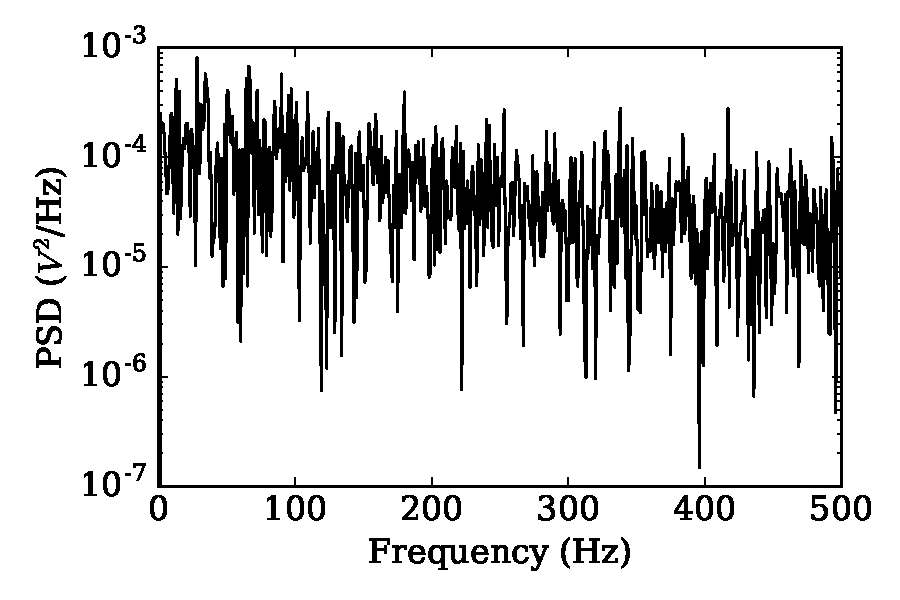
\includegraphics[width=\textwidth]{pics_iconip/psd_tau1.pdf}
			\caption{Spectrum analysis of (a).}
		\end{subfigure}
		\begin{subfigure}[t]{0.43\textwidth}
			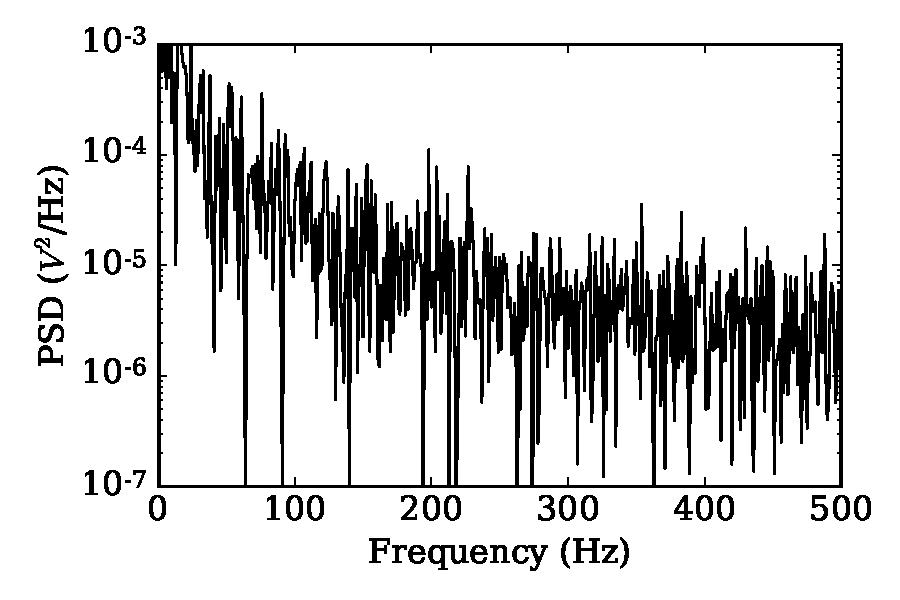
\includegraphics[width=\textwidth]{pics_iconip/psd_tau10.pdf}
			\caption{Spectrum analysis of (b).}
		\end{subfigure}\\
		\begin{subfigure}[t]{0.43\textwidth}
			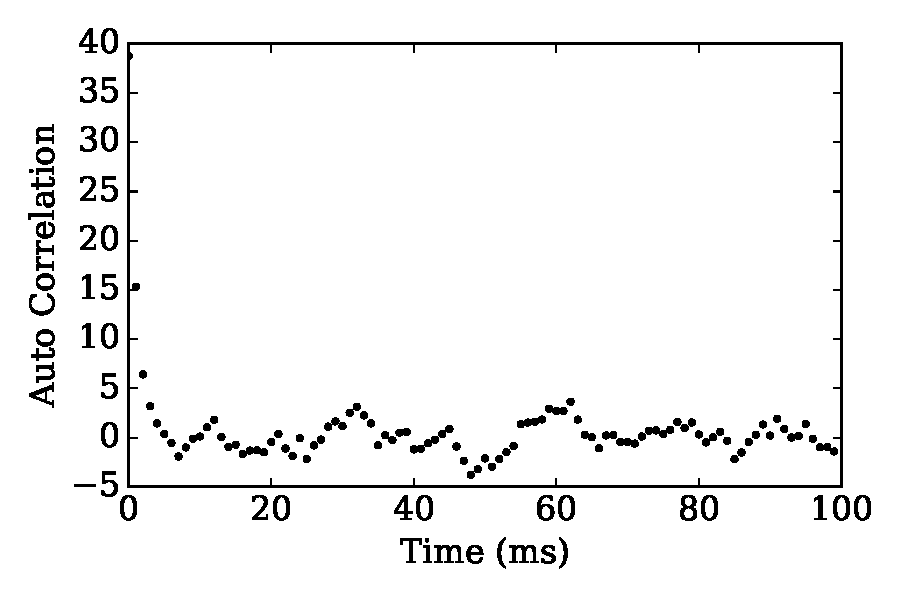
\includegraphics[width=\textwidth]{pics_iconip/autocorr_tau1.pdf}
			\caption{Autocorrelation of (a).}
		\end{subfigure}
		\begin{subfigure}[t]{0.43\textwidth}
			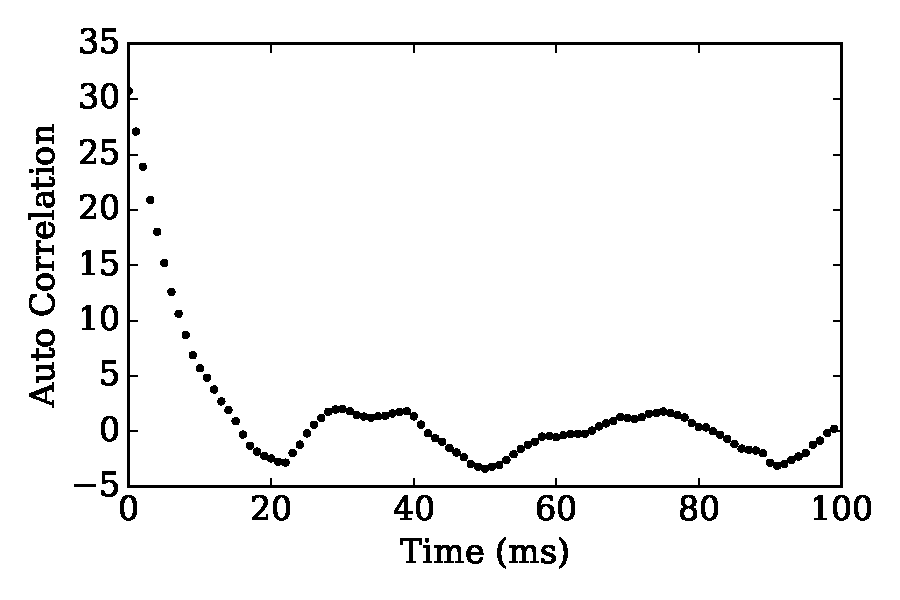
\includegraphics[width=\textwidth]{pics_iconip/autocorr_tau10.pdf}
			\caption{Autocorrelation of (b).}
		\end{subfigure}\\
		\begin{subfigure}[t]{0.43\textwidth}
			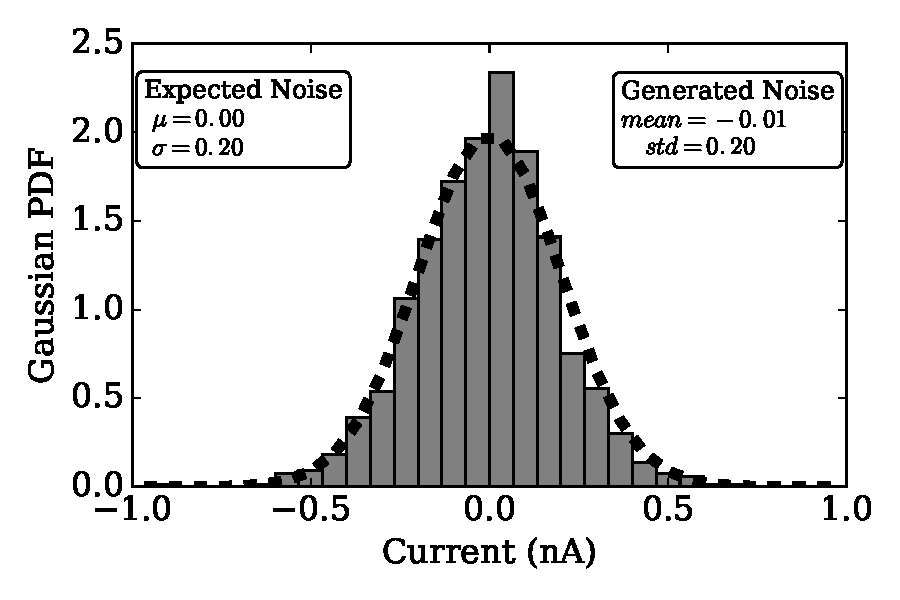
\includegraphics[width=\textwidth]{pics_iconip/distr_tau1.pdf}
			\caption{Distribution of samples of (a).}
		\end{subfigure}
		\begin{subfigure}[t]{0.43\textwidth}
			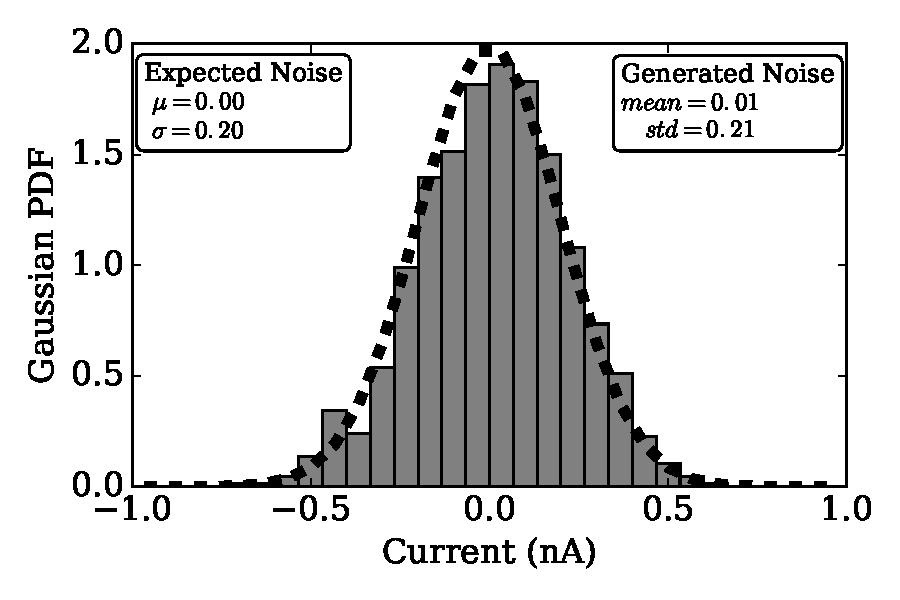
\includegraphics[width=\textwidth]{pics_iconip/distr_tau10.pdf}
			\caption{Distribution of samples of (b).}
		\end{subfigure}
		\caption{Noisy currents generated by 100 Poinsson spike trains to a LIF neuron with synaptic time constant $\tau_{syn}$=1~ms (left) and $\tau_{syn}$=10~ms (right). The currents are shown in time domain in (a) and (b), and spectrum domain in (c) and (d). The autocorrelation of both current signals are shown in (e) and (f). The distribution of the generated samples are plotted in bar chart to compare to the expected Gauss distribution, shown in (g) and (h).}
		\label{Fig:lif_pois}
	\end{figure}

	A more realistic simulation of a noisy current can be generated by 100 Poisson spike trains, 
	%assuming that large amount of small amplitude PSPs are required to reach the threshold and $\tau_syn$ limits to 0.
	where the mean and variance of the current are given by~\cite{la2008response}:
	\begin{equation}
	m_I = \tau_{syn}\sum_i w_i\lambda_{i}~, ~s_I^2=\frac{1}{2}\tau_{syn}\sum_i w_i^2\lambda_{i}~,
	\label{equ:distr0}
	\end{equation}
	where $\tau_{syn}$ is the synaptic time constant, and each Poisson spike train connects to the neuron with a strength of $w_i$ and a firing rate of $\lambda_i$.
	Two populations of Poisson spike sources, for excitatory and inhibitory synapses respectively, were connected to a single LIF neuron to mimic the noisy currents.
	The firing rates of the Poisson spike generators were determined by the given $m_I$ and $s_I$.
	Figures~\ref{Fig:spike_curr} illustrate the recorded firing rates responding to the Poissoin spike trains compared to the mean firing rate driven by \textit{NoisyCurrentSource} in Figure~\ref{Fig:current}.
	Note that the estimation of LIF response activity using the Siegert function requires noisy current with white noise, however
%	The use of noisy currents assumes that the post-synaptic potential (PSP) is a delta function, e.g. $\tau_{syn}$ tends to the limits of 0.
	in practice the release of neurotransmitter takes time ($\tau_{syn} >> 0$) and the synaptic current decays exponentially $I_{syn} = I_0 e^{\frac{-t}{\tau_{syn}}}$.
	Figures~\ref{Fig:lif_pois}~(a) and (b) show two examples of synaptic current of 0~nA mean and 0.2 standard deviation driven by 100 neurons firing at the same rate and with the same synaptic strength (half excitatory, half inhibitory), but of different synaptic time constant.
	Therefore, the current at any time $t$ during decaying period is dependant to the value at previous time step, which makes the synaptic current a coloured noise, see Figures~\ref{Fig:lif_pois}~(c) and (d).
%	and the noise added to the mean current is not white noise, but pink noise.
	
	We observe in Figure~\ref{Fig:spike_curr}~(a) that the response firing rate to synaptic current is higher than the \textit{NoisyCurrentSource} for all the 10 trials.
	This is caused by the coarse resolution (1~ms) of the spikes, thus the standard deviation of the current is larger than 0.2, shown in Figure~\ref{Fig:lif_pois}~(g);
	and the $\tau_{syn}$, even short as 1~ms, adds coloured noise instead of white noise to the current.
	However, Figure~\ref{Fig:lif_pois}~(h) shows a similar firing rate of both the synaptic driven current and the \textit{NoisyCurrentSource}, since both of the current signals have similar distribution and time correlation.
	Nevertheless, the analytical response function, Siegert formula, cannot approximate either of the practical simulations.
	
%	Thus the experiments show that a longer $\tau_{syn}$ increases the level of noise and widens the variance of the output firing rate.
	Although the use of Siegert function opened the door for modelling response activities of LIF neurons as activation function used in ANNs~\cite{Jug_etal_2012}, there are several drawbacks of this method:
	\begin{itemize}
		\item most importantly, the numerical analysis on an LIF response function is far from accurate in practice. `Practice' in the chapter means SNN simulations using LIF neurons.
		Thus the inaccurate model generates error between the estimation and the practical response firing rate.
%		This issue will be addressed in Section~\ref{subsec:practice}.
		
		
		\item the high complexity of the Siegert function causes much longer training time and more energy, let alone the high-cost computation on its derivative.
		%		\item the training uses Siegert function to estimate the output firing rate in the forward path, but uses the derivative of sigmoid function during back propagation for lower complexity.
		%		However, due to the difference between Siegert and sigmoid functions, error is introduced. 
		\item Siegert function is used to replace sigmoid functions for training spiking Restricted Boltzmann Machines~\cite{Jug_etal_2012}, thus neurons have to fire at high frequency (higher than half of the maximum firing rate) to represent the activation of a sigmoid unit and the network activity results in high power dissipation.
		\item better learning performance has been reported using ReLU, so modelling ReLU-like activation function for spiking neurons is needed.  
	\end{itemize}
	
	Therefore, we propose the NSP function which provides solutions to the drawbacks of Siegert unit.

		
	\subsection{Noisy Softplus~(NSP)}
	\label{sec:NSP}
%	Due to the limited time resolution of common SNN simulators and the time taken for neurotransmitter release, $\tau_{syn}$, mismatches exist between the analytical response function, the Siegert formula, and practical neural activities.
%	Consequently, a unified activation function is required to model the practical responses of a LIF neuron.
%	Inspired by the set of response functions triggered by different levels of noise, we propose the NSP activation function:
%	\begin{equation}
%	y = f_{ns}(x, \sigma) = k \sigma \log [1 + \exp(\frac{x}{k \sigma})],
%	\label{equ:nsp}
%	\end{equation}
%	where $x$ refers to the mean current, $y$ indicates the strength of the output firing rate, $\sigma$ plays an important role to define the noise level, and $k$, which is determined by the neuron parameters, controls the shape of the curves.
%	Note that the novel activation function we propose contains two parameters, the current and its noise, which can be estimated by Equation~\ref{equ:distr0}:
%	\begin{equation}
%	x = \tau_{\textit{\textrm{syn}}}\sum_i w_i\lambda_{i}~, ~\sigma^2=\frac{1}{2}\tau_{\textit{\textrm{syn}}}\sum_i w_i^2\lambda_{i}~,
%	\label{equ:distr}
%	\end{equation}
%	where $\lambda_i$ indicates the firing rate of an input spike train.
%	Figure~\ref{fig:nsp} shows the activation function in curve sets corresponding to different discrete noise levels, and in a 3D plot.
%	\begin{figure}[thb!]
%		\centering
%		\begin{subfigure}[t]{0.4\textwidth}
%			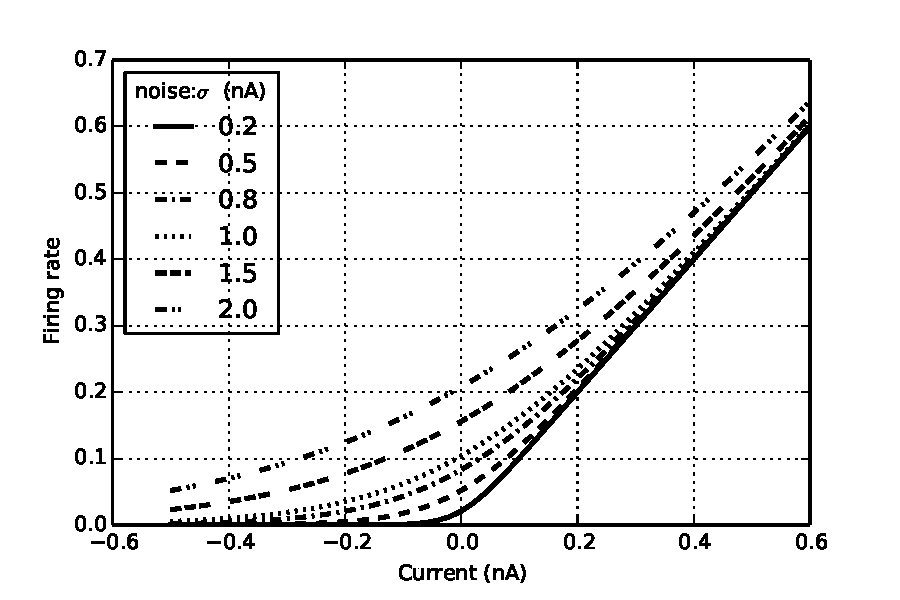
\includegraphics[width=\textwidth]{pics_iconip/4.pdf}
%			\caption{Noisy Softplus}
%		\end{subfigure}
%		\begin{subfigure}[t]{0.4\textwidth}
%			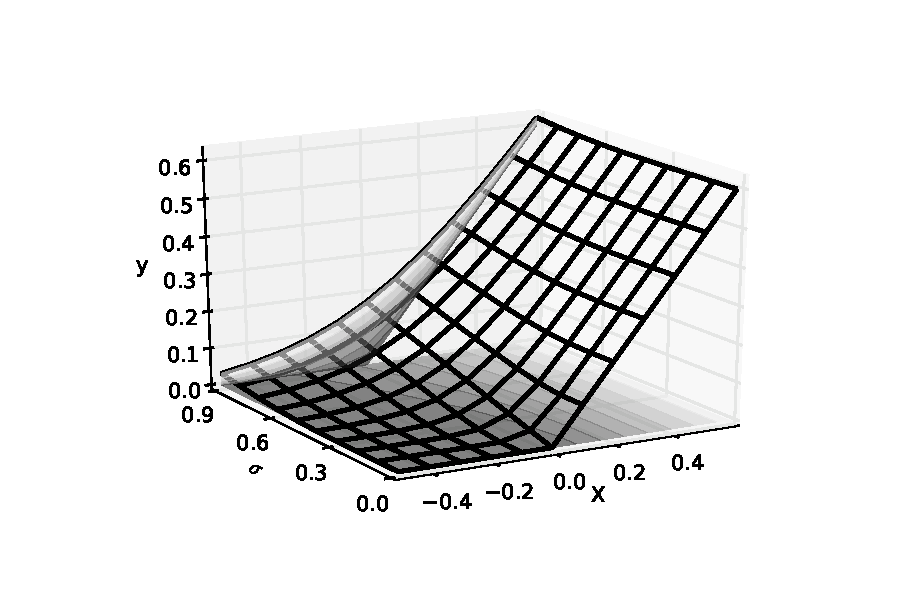
\includegraphics[width=\textwidth]{pics_iconip/5.pdf}
%			\caption{Noisy Softplus in 3D}
%		\end{subfigure}
%		\caption{
%			Noisy Softplus fits to the response function of the LIF neuron.
%			Noisy Softplus in (a) curve sets and (b) 3D.}
%		\label{fig:nsp}
%	\end{figure}	
%	
%	The derivative is the logistic function scaled by $k\sigma$:
%	\begin{equation}
%	\frac{\partial f_{ns}(x,\sigma)}{\partial x} = \frac{1}{1+exp(-\frac{x}{k\sigma})}~~,
%	\label{equ:logist}
%	\end{equation}	
%	which could be easily applied to back propagation in any network training.
%	However, such a derivative function of low complexity does not present in Siegert function.
	Due to the limited time resolution of common SNN simulators and the time taken for neurotransmitter release, $\tau_{syn}$, mismatches exist between the analytical response function, the Siegert formula, and practical neural activities.
	Consequently to model the practical responses of LIF neurons (see Figure~\ref{fig:nsp}(a)) whose output firing rates are determined by the mean and variance of the noisy input currents, the NSP was proposed:
	\begin{equation}
	y = f_{ns}(x, \sigma) = k \sigma \log [1 + \exp(\frac{x}{k \sigma})]~,
	\label{equ:nsp}
	\end{equation}
	where $x$ and $\sigma$ refer to the mean and standard deviation of the input current, $y$ indicates the intensity of the output firing rate, and $k$, determined by the biological configurations on the LIF neurons~\cite{liu2016noisy}~(listed in Table~\ref{tbl:pynnConfig}), controls the shape of the curves.
	Note that the novel activation function we proposed contains two parameters, the mean current and its noise, which can be estimated by Equation~\ref{equ:distr0}:
	\begin{equation}
	x = \tau_{\textit{\textrm{syn}}}\sum_i w_i\lambda_{i}~, ~\sigma^2=\frac{1}{2}\tau_{\textit{\textrm{syn}}}\sum_i w_i^2\lambda_{i}~,
	\label{equ:distr}
	\end{equation}
	where $\lambda_i$ indicates the firing rate of an input spike train.
	%; both are naturally obtained in spiking neurons.
	% With doubled information, more powerful training methods and network models are expected. 
	\begin{figure}[thb!]
		\centering
		\begin{subfigure}[t]{0.48\textwidth}
			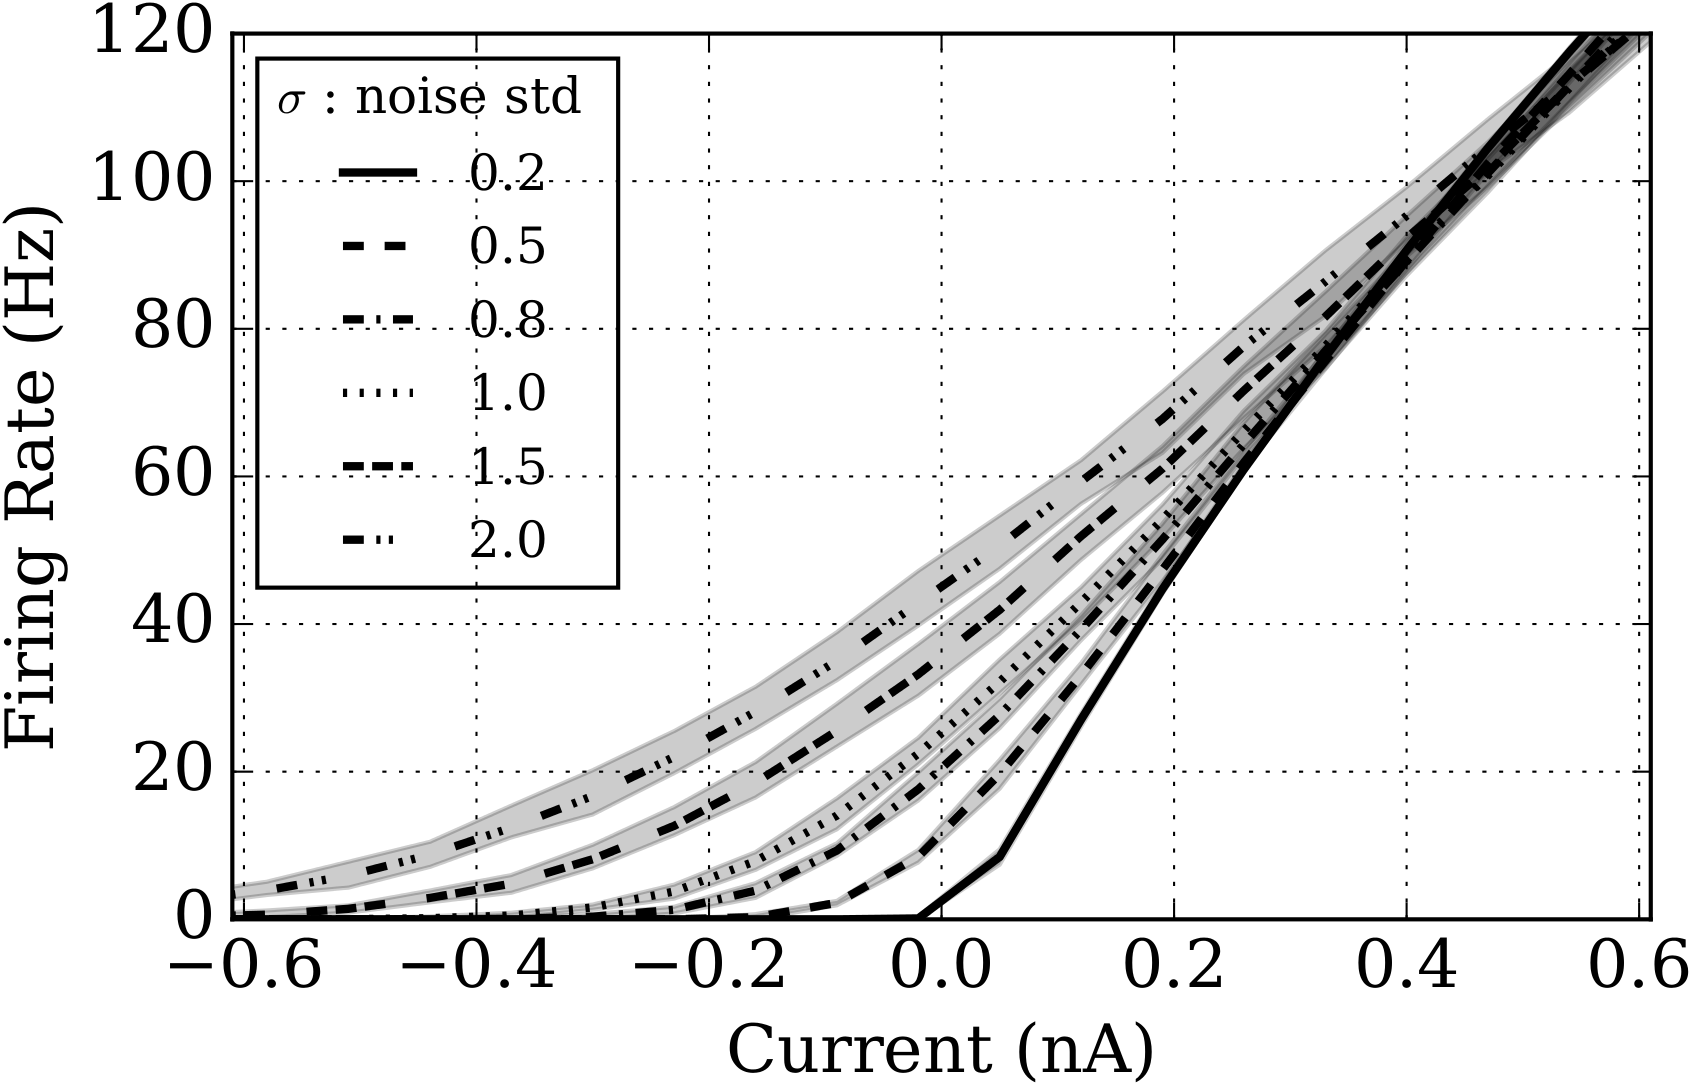
\includegraphics[width=\textwidth]{pics_iconip/siegert.png}
			\caption{Response firing rate of an LIF neuron}
		\end{subfigure}
		\begin{subfigure}[t]{0.48\textwidth}
			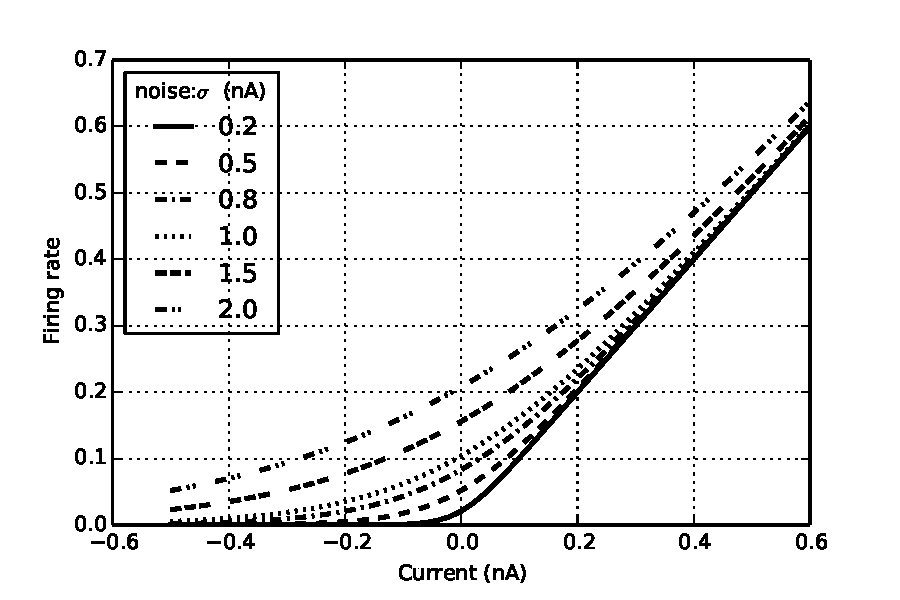
\includegraphics[width=\textwidth]{pics_iconip/4.pdf}
			\caption{NSP}
		\end{subfigure}
		\caption{
			%		NSP fits to the response function of the LIF neuron.
			NSP models the LIF response function.
			(a) Firing rates measured by simulations on an LIF neuron driven by different input currents and discrete noise levels.
			Bold lines show the average and the grey colour fills the range between the minimum and the maximum.
			(b) NSP activates the input $x$ according to different noise levels where $k=0.16$.}
		\label{fig:nsp}
	\end{figure}
	
	Figure~\ref{fig:nsp}(b) shows the activation function in curve sets corresponding to different discrete noise levels which mimics the responding activities of practical simulations of LIF neurons, shown in Figure~\ref{fig:nsp}(a).
	Since the NSP takes two variables as inputs, the activation function can be plotted in 3D, see Figure
	
	\begin{figure}[bt]
		\centering
		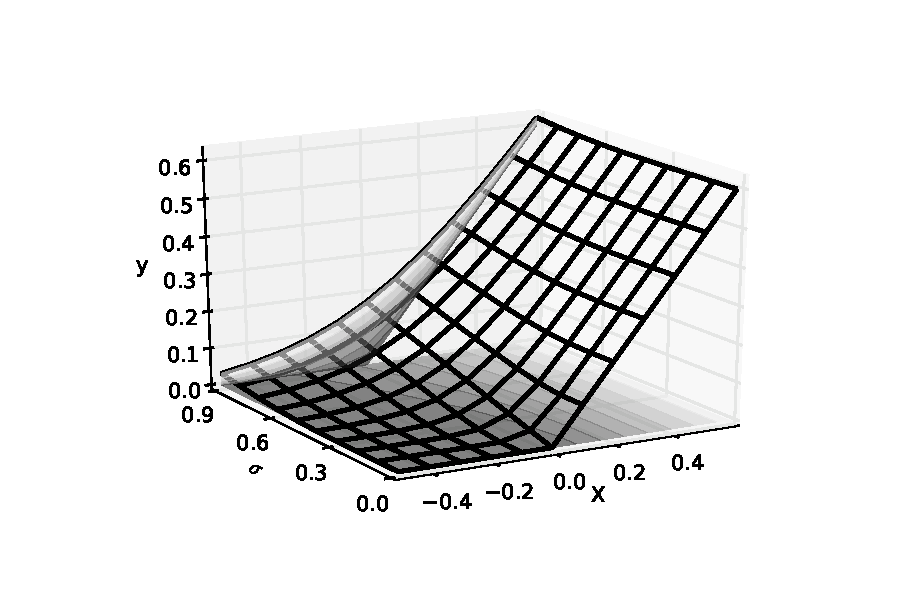
\includegraphics[width=0.7\textwidth]{pics_iconip/5.pdf}
		\caption{Noisy Softplus in 3D.}
		\label{Fig:NSP3D}
	\end{figure}

	The derivative of the NSP is the logistic function scaled by $k\sigma$:
	\begin{equation}
	\frac{\partial f_{ns}(x,\sigma)}{\partial x} = \frac{1}{1+exp(-\frac{x}{k\sigma})}~~,
	\label{equ:logist}
	\end{equation}	
	which could be applied easily to back propagation in any ANN training.	
	
	
\section{Generalised Off-line SNN Training}
\label{sec:genrial_SNN}
%	We have discussed modelling response firing activity of a LIF neuron with a unified activation function, Noisy Softplus.
%	However the demonstration of mapping the physical activity to numerical ANN calculations is still required to train the layered-up deep network.
%	
%	\subsection{Equivalent Input and Output}
%	
%	\begin{figure}[bt]
%		\centering
%		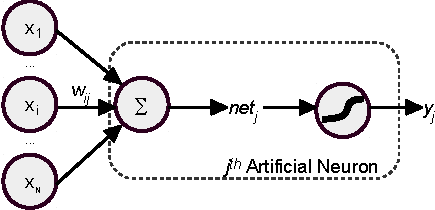
\includegraphics[width=0.7\textwidth]{pics_iconip/neuron.pdf}
%		\caption{Artificial neuron model in ANNs. }
%		\label{Fig:neuron}
%	\end{figure}
%	Neurons in ANNs take inputs from their previous layer, and feed the weighted sum of their input, $net_j = \sum_i w_{ij}x_i$, to the activation function.
%	The transformed signal then forms the output of an artificial neuron, $y_j=f(net_j)$, see Figure~\ref{Fig:neuron}.	
%	However, Noisy Softplus takes physical quantities of current, and firing rate as input/output, thus an extra step is still needed to map the firing rate to numerical values in ANNs.
%	According to Equation~\ref{equ:distr}, the mean of the current feeding into a spiking neuron is equivalent to $net$ of artificial neurons, where
%	\begin{equation}
%	\begin{aligned}
%		& {m_I}_j = \sum_i w_{ij}(\lambda_{i}\tau_{syn})~, \textrm{  then}\\
%		& net_j= \sum_i w_{ij} x_i~~, \textrm{~~and~~}
%		x_i = \lambda_{i}\tau_{syn}~.
%	\end{aligned}
%	\label{equ:mi_input}
%	\end{equation}
%	The noise level of Noisy Softplus, $\sigma^2$, is the variance of the current, which also can be seen as a weighted sum of the same input $x$ but with different weights:
%	\begin{equation}
%	\begin{aligned}
%		& {s_I^2}_j=\sum_i(\frac{1}{2} w_{ij}^2) (\lambda_{i}\tau_{syn})~, \textrm{  then}\\
%		& \sigma^2_j= \sum_i (\frac{1}{2} w_{ij}^2) x_i~~.
%	\end{aligned}
%	\label{equ:si_input}
%	\end{equation}
%	
%	\begin{figure}[bt!]
%		\centering
%		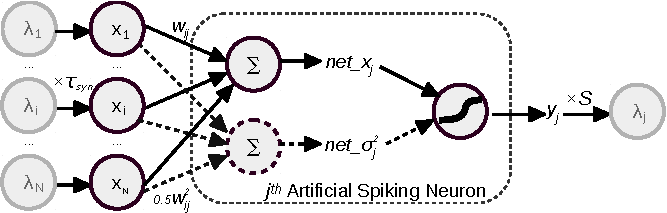
\includegraphics[width=0.98\textwidth]{pics_iconip/neuron_o.pdf}
%		\caption{Artificial spiking neuron takes scaled firing rates as input, then transforms weighted sum in some activation unit to its output which can be scaled-up to the firing rate of an output spike train.}
%		\label{Fig:sneuron}
%	\end{figure}
%	
%	Noisy Softplus transforms the noisy current with parameters of $(net_j, \sigma_j)$ to the equivalent ANN output $y_j$ , where it can be scaled up by the factor $S$ to the firing rate of SNNs.
%	Note that the calculation of noise level is not necessary for activation functions other than Noisy Softplus, for example, it can be set to a constant for Softplus or 0 for ReLU.
%	We name the neuron model `artificial spiking neurons' which takes firing rates of spike trains as input and output. 
%	The entire artificial spiking neuron model is then generalised to any ReLU/Softplus-like activation functions, See Figure~\ref{Fig:sneuron}.
%	
%
%	
%	
%	\subsection{Layered-up Network}
%	\label{subsec:ns_train}
%%	Figure~\ref{Fig:sneuron} shows an complete transformation process of a spiking neuron, which mimics the biological neurons taking and generating spike trains.
%	Referred to Figure~\ref{Fig:sneuron}, if we move the left end process of $\times \tau_{syn}$ to the right end after $\lambda_j$, Figure~\ref{Fig:sneuron} forms the same model structure as artificial neurons shown in Figure~\ref{Fig:neuron}: neurons take $x$ as input and outputs $y$, and this conversion is illustrated in Figure~\ref{Fig:tneuron}.
%	The process within such an artificial neuron is divided into weighted summation and activation, which also applies to SNN modelling by combining the scaling factor $S$ and the synaptic time constant $\tau_{syn}$ to activation functions.
%	Thus the combined activation function for modelling SNNs should be:
%	\begin{equation}
%	y = f(x) \times S \times \tau_{syn}~~,
%	\label{equ:full_act}
%	\end{equation}
%	and its derivative function which is used when back propagates is:
%	\begin{equation}
%	\frac{\partial y}{\partial x} = f'(x) \times S \times \tau_{syn}~~.
%	\end{equation}
%	
%	\begin{figure}[tbh!]
%		\centering
%		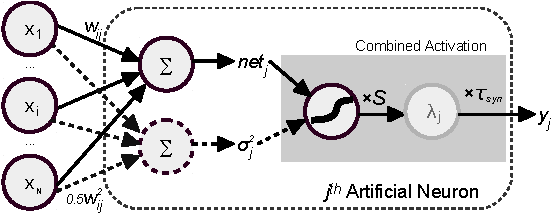
\includegraphics[width=0.8\textwidth]{pics_iconip/neuron_t.pdf}
%		\caption{Transforming artificial spiking neurons to artificial neurons for SNN modelling. The combined activation links the firing activity of a spiking neuron to the numerical value of ANNs.}
%		\label{Fig:tneuron}
%	\end{figure}
%	
%	
%	
%
%	
%
%	
%	Thus, using this method of ANN-trained SNNs, the activation functions are of lower complexity than the Siegert formula, and their corresponding derivative functions can be directly used for back propagation.
%	Furthermore, the method enables ReLU-like activation functions for SNN training, thus improving the recognition accuracy while keeping a relative lower firing rate compared to sigmoid neurons. 
%	Most significantly, the ANN-trained weights are ready for use in SNNs without any transformation, and the output firing rate of a spiking neuron can be estimated in the ANN simulation.
%	
%	
%	\subsection{Fine Tuning}
%	There are two aspects to the fine tuning which makes the ANN closer to SNNs:
%	Firstly, using Noisy Softplus activation functions in a whole trained network operates every single neuron running in a similar noise level as in SNNs, thus the weights trained by other activation functions will be tuned to fit closer to SNNs.
%	Secondly, the output firing rate of any LIF neuron is greater than zero as long as noise exists in their synaptic input.
%	Thus adding up a small offset on the labels directs the model to approximate to practical SNNs. 
%	
%	The labels of data are always converted to binary values for ANN training.
%	This enlarges the disparities between the correct recognition label and the rest to train the network for better classification capability.
%	Consequently, we train the network as stated in Section~\ref{subsec:ns_train} with any activation function and then fine-tune it with Noisy Softplus to take account of both accuracy and practical network activities of SNNs.
%	However, we add a small number, for example 0.01, to all the binary values of the data labels.
%	Doing so helps the training to loosen the strict objective function to predict exact labels with binary values.
%	Instead, it allows a small offset to the objective.
%	An alternative method is to use Softmax function at the top layer, which aims to map real vectors to the range of $(0,1)$ that add up to 1. 
%	However, without a limit on the input of Softmax, it will be easy to reach or even exceed the highest firing rate of a spiking neuron.
%	The result of fine tuning on a ConvNet will be demonstrated in Section~\ref{subsec:result_compare}.
	
	\subsection{Mapping NSP to Concrete Physical Units}
	\label{sec:af_model}
	The inputs of the NSP, $x$ and $\sigma$, are obtained from physical variables as stated in Equation~\ref{equ:distr}, thus they are already in physical units (nA).
	Therefore, linearly scaling up the activation function by a factor~$S$~(Hz~/~nA) can approximate the output firing rate $\lambda_{\textit{\textrm{out}}}$ of an LIF neuron in Hz:
	\begin{equation}
	\lambda_{\textit{\textrm{out}}} \simeq f_{ns}(x, \sigma) \times S = k \sigma \log [1 + \exp(\frac{x}{k \sigma})] \times S~.
	\label{equ:fit}
	\end{equation}	
	
	
	Suitable calibrations of $k$ and $S$ in Equation~\ref{equ:fit} enables NSP to closely match the practical response firing rates of LIF neurons given various biological parameters.
	The parameter pair of $(k, S)$ is curve-fitted with the triple data points of $(\lambda_{\textit{\textrm{out}}}, x, \sigma)$ and the calibration currently is conducted by linear least squares regression.
	The output firing rate $\lambda_{\textit{\textrm{out}}}$ is measured from SNN simulations where an LIF neuron is driven by synaptic input current of Poisson spike trains.
	Figure~\ref{Fig:nsptau1} shows two calibration results in which the parameters were fitted to $(k, S)=(0.19,208.76)$ when the synaptic constant is set to $\tau_{\textit{\textrm{syn}}}=1$~ms and was fitted to $(k, S)=(0.35,201.06)$ when $\tau_{\textit{\textrm{syn}}}=10$~ms.
	%numerical analysis is considered however for future work to express the factors with biological parameters of an LIF neuron.
	
	\begin{figure}
		\centering
		\begin{subfigure}[t]{0.48\textwidth}
			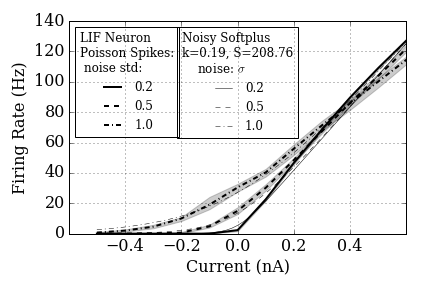
\includegraphics[width=\textwidth]{pics_iconip/4-1.png}
			\caption{$\tau_{\textit{\textrm{syn}}}$=1~ms}
		\end{subfigure}
		\begin{subfigure}[t]{0.48\textwidth}
			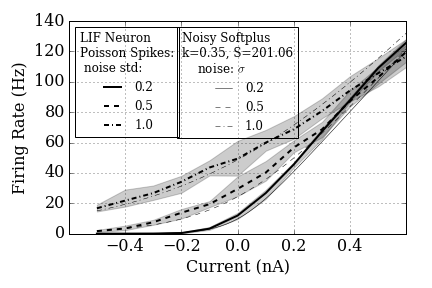
\includegraphics[width=\textwidth]{pics_iconip/4-10.png}
			\caption{$\tau_{\textit{\textrm{syn}}}$=10~ms}
		\end{subfigure}
		\caption{NSP fits to the response firing rates of LIF neurons in concrete physical units.
			Recorded response firing rate of an LIF neuron driven by synaptic current with two synaptic time constants: (a) $\tau_{\textit{\textrm{syn}}}$=1~ms and (b) $\tau_{\textit{\textrm{syn}}}$=10~ms. Averaged firing rates of simulation trails are shown in bold lines, and the grey colour fills the range between the minimum to maximum of the firing rates. The thin lines are the scaled NSP.}
		\label{Fig:nsptau1}
	\end{figure}
	
	\subsection{Parametric Activation Functions~(PAFs)}
	\begin{figure}[tbh!]
		\centering
		\begin{subfigure}[t]{0.7\textwidth}
			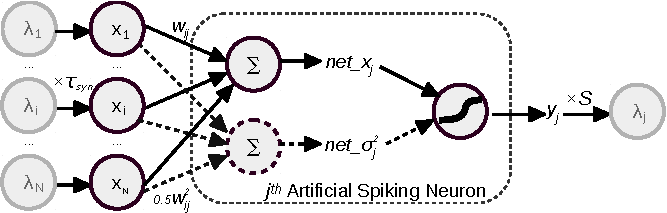
\includegraphics[width=\textwidth]{pics_iconip/neuron_o.pdf}
			\caption{An artificial spiking neuron modelled by NSP.}
		\end{subfigure}\\
		\begin{subfigure}[t]{0.7\textwidth}
			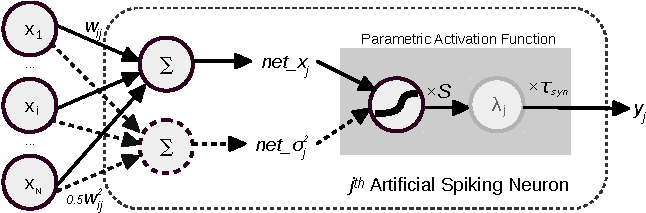
\includegraphics[width=\textwidth]{pics_iconip/neuron_PAF.pdf}
			\caption{An artificial spiking neuron modelled by PAF-NSP.}
		\end{subfigure}
		\caption{The PAF links the firing activity of a spiking neuron to the numerical value of ANNs.}
		\label{Fig:tneuron}
	\end{figure}
	
	
	Neurons in ANNs take inputs from their previous layer, and feed the weighted sum of their input, $net_j = \sum_i w_{ij}x_i$, to the activation function.
	The transformed signal then forms the output of an artificial neuron, which can be denoted as $y_j=f(net_j)$, see Figure~\ref{Fig:compare_as}(a).
	However, a spiking neuron modelled by NSP takes the firing rate as its input/output, thus Equation~\ref{equ:distr} can be written as:
	\begin{equation}
	net_j = \sum_i w_{ij}(\lambda_{i}\tau_{\textit{\textrm{syn}}})~,
	~\sigma^2_j= \sum_i (\frac{1}{2} w_{ij}^2)(\lambda_{i}\tau_{\textit{\textrm{syn}}})~, 
	% \textrm{~~and~~} x_i = \lambda_{i}\tau_{\textit{\textrm{syn}}}~.
	\label{equ:mi_input}
	\end{equation}
	and input $ x_i $ of an artificial neuron can be seen as $x_i=\lambda_{i}\tau_{\textit{\textrm{syn}}}$, see Figure~\ref{Fig:tneuron}(a).
	
	
	If instead of multiplying every input by $\tau_{\textit{\textrm{syn}}}$ (left of Fig.~\ref{Fig:tneuron}(a)) we do it in every output after $\lambda_j$, (right of Fig.~\ref{Fig:tneuron}(b)) we obtain the same neuron model and structure as a typical neuron in ANNs, See Figure~\ref{Fig:compare_as}(a), that neurons take $x$ as input and output $y$.
	%	The PAF version of the activation function (Eq.~\ref{equ:PAF}) will be linearly-scaled by the conversion parameter $S$ and the synaptic time constant $\tau_{syn}$:
	The only difference lies in the activation function where the artificial spiking neuron takes PAF, which is a simple linearly-scaled activation function with a parameter $p$, which is determined by the product of the scaling parameter $S$ and the synaptic time constant $\tau_{\textit{\textrm{syn}}}$:
	
	\begin{equation}
	y = p \times f(x) = S \times \tau_{\textit{\textrm{syn}}} \times f(x)~,
	\label{equ:PAF}
	\end{equation}
	and its derivative function, which is used for back propagation, is:
	\begin{equation}
	\frac{\partial y}{\partial x} = p \times f'(x) = S \times \tau_{\textit{\textrm{syn}}} \times f'(x)~.
	\end{equation}
	
	Excitingly, PAF not only allows NSP to model spiking LIF neurons on ANNs, once the parameter $p$ is acquired the PAF can be generalised to other activation functions.
	Note that the calculation of noise level is not necessary for other activation functions, for example, it can be set to a constant for Softplus or 0 for ReLU.
	\subsection{Generalised SNN Training}
	\label{subsec:ns_train}
	
	The simple change on activation functions presented in the previous section allows the use of common ANN training methods to obtain SNN-compatible weights.
	Consequently, training SNNs can be done in three simple steps: 
	\begin{enumerate}
		\item Calibrate the parameters $(k, S)$ for Noisy Softplus which models response firing rates of LIF neurons, thus to estimate parameter $p=S \times \tau_{\textit{\textrm{syn}}}$ for PAFs. Since $(k, S)$ are solely dependent on the biological configurations of an LIF neuron, the same $p$ can be used for different activation functions and network architectures.
		\item Train any feed-forward ANN with a PAF version of an activation function.
		Training compatibility allows us to choose computationally simple activation functions to increase training speed.
		%		Surprisingly, the use of PAF-ReLU provides the best accuracy scores for an SNN on the MNIST dataset. 
		\item Transfer the weights directly to the SNN, which should use the same LIF characteristics used in Step 1.
	\end{enumerate}
	
	\subsection{Fine Tuning}
	We can train the network with any PAF as stated above, and then fine-tune it with PAF-NSP in the hope of improving the performance of the equivalent SNN by closely modelling the spiking neurons with NSP.
	%	both the learning performance provided by ReLU and practical network activities of SNNs modelled by NSP.
	Additionally, we add a small number, for example 0.01, to all the binary values of the labels on the training data.
	Although binary labels enlarges the disparities between the correct recognition label and the rest for better classification capability, 
	spiking neurons seldom stay silent even with negative current influx, thus setting labels to 0 are not practical for training SNNs.
	Therefore, adding an offset relaxes the strict objective function of predicting exact labels with binary values.
	%	Instead, it allows a small offset to the objective.
	%	An alternative method is to use Softmax function at the top layer, which aims to map real vectors to the range $(0,1)$ that add up to 1. 
	%	However, without a limit on the input of Softmax, it will be easy to reach or even exceed the highest firing rate of a spiking neuron.
	
	
	There are two aspects to the fine tuning which make the ANN closer to SNNs:
	Firstly, using the NSP activation functions causes every single neuron to run as a similar noise level as in SNNs, thus the weights trained by other activation functions will be tuned to fit closer to SNNs.
	Secondly, the output firing rate of any LIF neuron is greater than zero as long as noise exists in their synaptic input.
	Thus adding up a small offset on the labels directs the model to approximate practical SNNs. 
	The result of fine tuning on a ConvNet will be demonstrated in Section~\ref{subsec:result_compare}.
	
\section{Results}
\label{sec:iconipResult}
	\subsection{Experiment Description}
	% Architecture
	A spiking ConvNet was trained on MNIST~\cite{lecun1998gradient} dataset, 
	%a popular database in neuromorphic vision, 
	using the generalised SNN training method stated above.
	The architecture (784-6c-6p-12c-12p-10fc illustrated in Section~\ref{sec:convnet}) contains $28\times28$ input units, followed by two convolution-pooling layers with 6 and 12 convolutional kernels each, and 10 output neurons fully connected to the last pooling layer to represent the classified digit.
	
	% Training
	To train the ConvNet, firstly, we estimated parameter $p$ for PAFs given LIF configurations listed in Talbe~\ref{tbl:pynnConfig} and $\tau_{\textit{\textrm{syn}}}=5$~ms, $p = S \times \tau_{\textit{\textrm{syn}}} = 1.005$, where $(k=0.30, S=201)$ were calibrated using NSP. 
	Secondly, the training employed PAFs with three core activation functions: ReLU, Softplus and NSP to compare their learning and recognition performance.
	%	The parameter $p$ was estimated as $p = S \times \tau_{\textit{\textrm{syn}}} = 1.005$ by calibrating the NSP with LIF response firing rate: $(k=0.30, S=201)$ given $\tau_{\textit{\textrm{syn}}}=5 ms$.
	%	The pixel intensities of the input images were normalised to 100~Hz to represent the firing rates of the input spikes.
	The weights were updated using a decaying learning rate, 50 images per batch and 20 epochs.
	Finally, the trained weights were then directly transferred to the corresponding spiking ConvNets for recognition test on the SNN simulator, NEST~\cite{gewaltig2007nest}.
	To validate the effect of fine tuning, we took another training epoch to train these models with PAF-NSP with data labels shifted by $+0.01$.
	Then the weights were also tested on SNN simulations to compare with the ones before fine-tuning.
	
	%	The recognition test took the whole testing dataset of MNIST which contains $10,000$ images.
	At the testing stage, the input images were converted to Poisson spike trains~\cite{liu2016bench} and presented for 1~s each.
	The output neuron which fired the most indicated the classification of an input image.
%	
%	A convolutional network model was trained on MNIST,
%	%	~\cite{lecun1998gradient}
%	a popular database in neuromorphic vision, using the ANN-trained SNN method stated above.
%	The architecture contains $28\times28$ input units, followed by two convolutional layers 6c5-2s-12c5-2s, and 10 output neurons fully connected to the last pooling layer to represent the classified digit.
%	The detailed network structure and training procedure can be found in Section~\ref{sec:convnet}.
%	
%	The training only employed Noisy Softplus units that all the convolution, average sampling, and the fully-connected neurons use Noisy Softplus function with no bias.
%	The parameters of the activation function were calibrated as, $(k=0.30, S=201)$,  for LIF neurons~(see~Tablel~\ref{tbl:pynnConfig}) of $\tau_{syn}=5$~ms.
%	The input images were scaled by 100~Hz to present the firing rates of input spikes.
%	The weights were updated using a decaying learning rate, 50 images per batch and 20 epochs.
%	The ANN-trained weights were then directly applied in the corresponding convolutional SNN without any conversion for recognition tasks.
%	Figure~\ref{Fig:spike_ConvNet} illustrates the working scheme of a spiking version of convolution and pooling neurons.
%	\begin{figure}[bt]
%		\centering
%		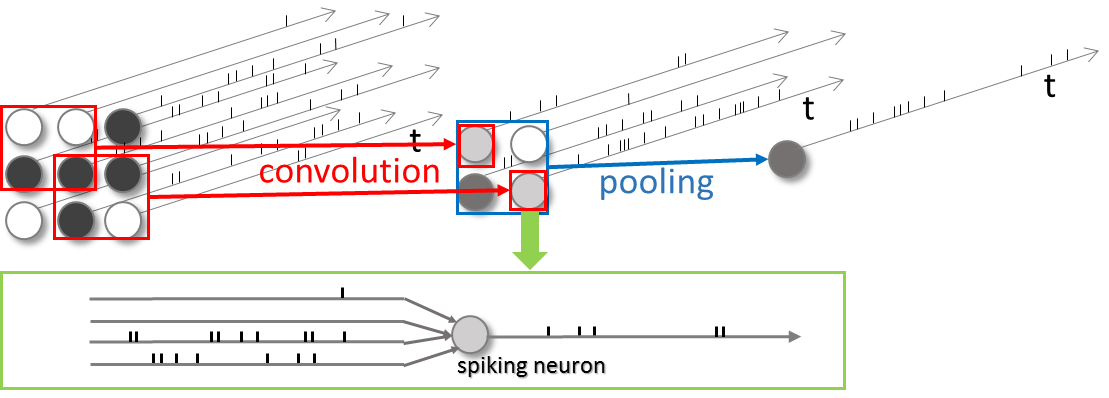
\includegraphics[width=0.95\textwidth]{pics_iconip/spike_conv.png}
%		\caption{Spike neurons work in convolution and pooling layers, whose firing rates of the spike train represents the intensities of neural activations.}
%		\label{Fig:spike_ConvNet}
%	\end{figure}
	
	
	\subsection{Neural Activity}
%	To validate how well the Noisy Softplus activation fits to the response firing rate of LIF neurons in a real application, we simulated the model on NEST~\cite{gewaltig2007nest} using the Poisson MNIST dataset~\cite{liu2016bench} and the neurons of a convolutional map were observed.
	To validate how well the NSP activation fits to the response firing rate of LIF neurons in SNNs, we simulated one of the PAF-NSP trained ConvNets on NEST.
	%	A small test consisted of ten MNIST digits presented as Poisson spike trains for 1~s each.
	Ten testing images were convolved with a trained $5\times5$ kernel, and the output firing rates of the spiking neurons were recorded, see Figure~\ref{fig:cnn} and compared to the predictions of these PAFs: $\lambda' = S \times f(x) = y/\tau_{\textit{\textrm{syn}}}$, see Figure~\ref{fig:af_compare}.
	
		\begin{figure}[htbp!]
		\centering
		\begin{subfigure}[t]{0.65\textwidth}
			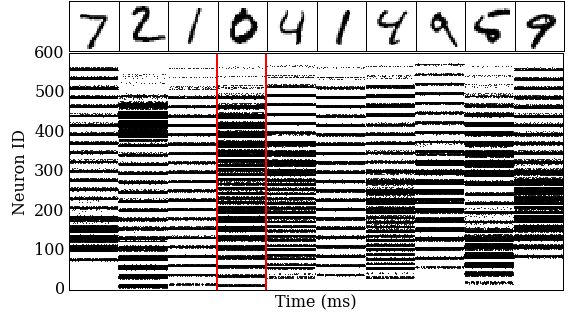
\includegraphics[width=\textwidth]{pics_iconip/6-1.png}
			\caption{10 input digits presented in Poisson spike trains.}
			\label{Fig:61}
		\end{subfigure}\\
		\begin{subfigure}[t]{0.3\textwidth}
			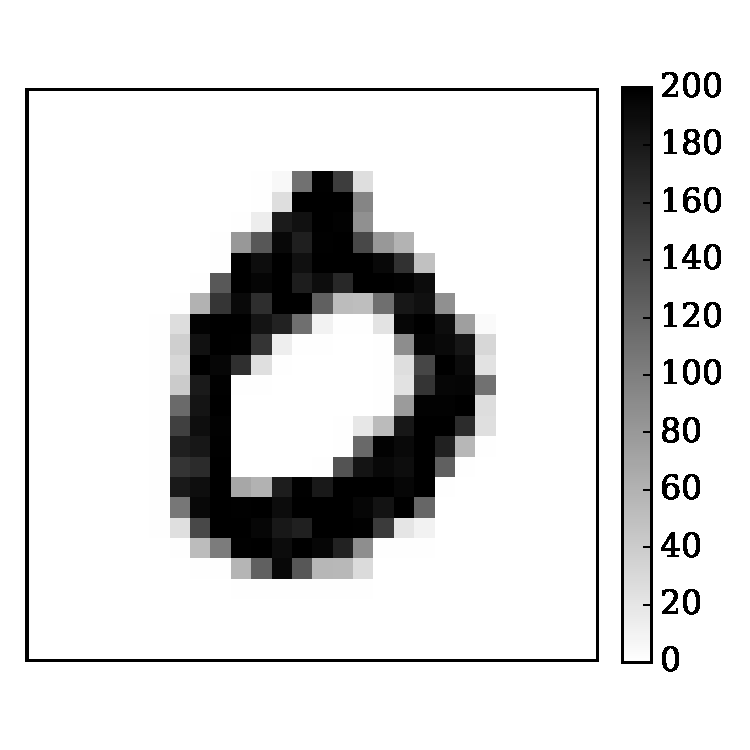
\includegraphics[width=\textwidth]{pics_iconip/6-2.pdf}
			\caption{Pixel firing rates.}
			\label{Fig:62}
		\end{subfigure}
		\begin{subfigure}[t]{0.3\textwidth}
			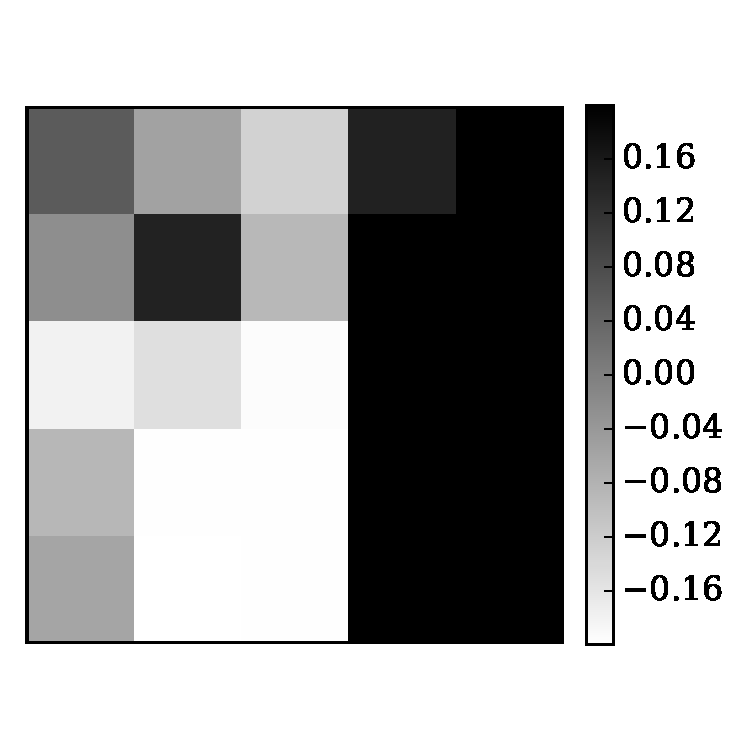
\includegraphics[width=\textwidth]{pics_iconip/6-3.pdf}
			\caption{5x5 kernel.}
			\label{Fig:63}
		\end{subfigure}
		\begin{subfigure}[t]{0.3\textwidth}
			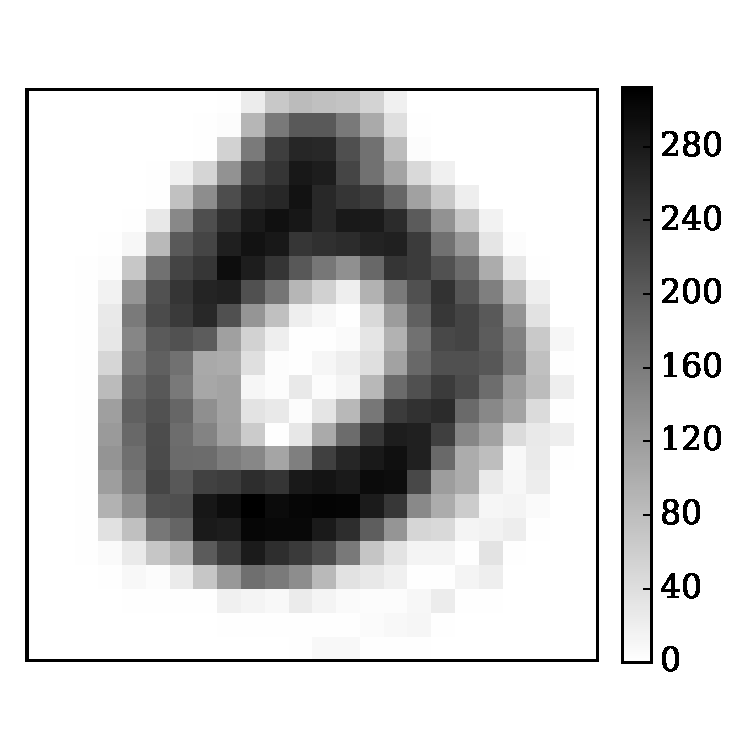
\includegraphics[width=\textwidth]{pics_iconip/6-4.pdf}
			\caption{Convolved output.}
			\label{Fig:64}
		\end{subfigure}\\
		\begin{subfigure}[t]{0.5\textwidth}
			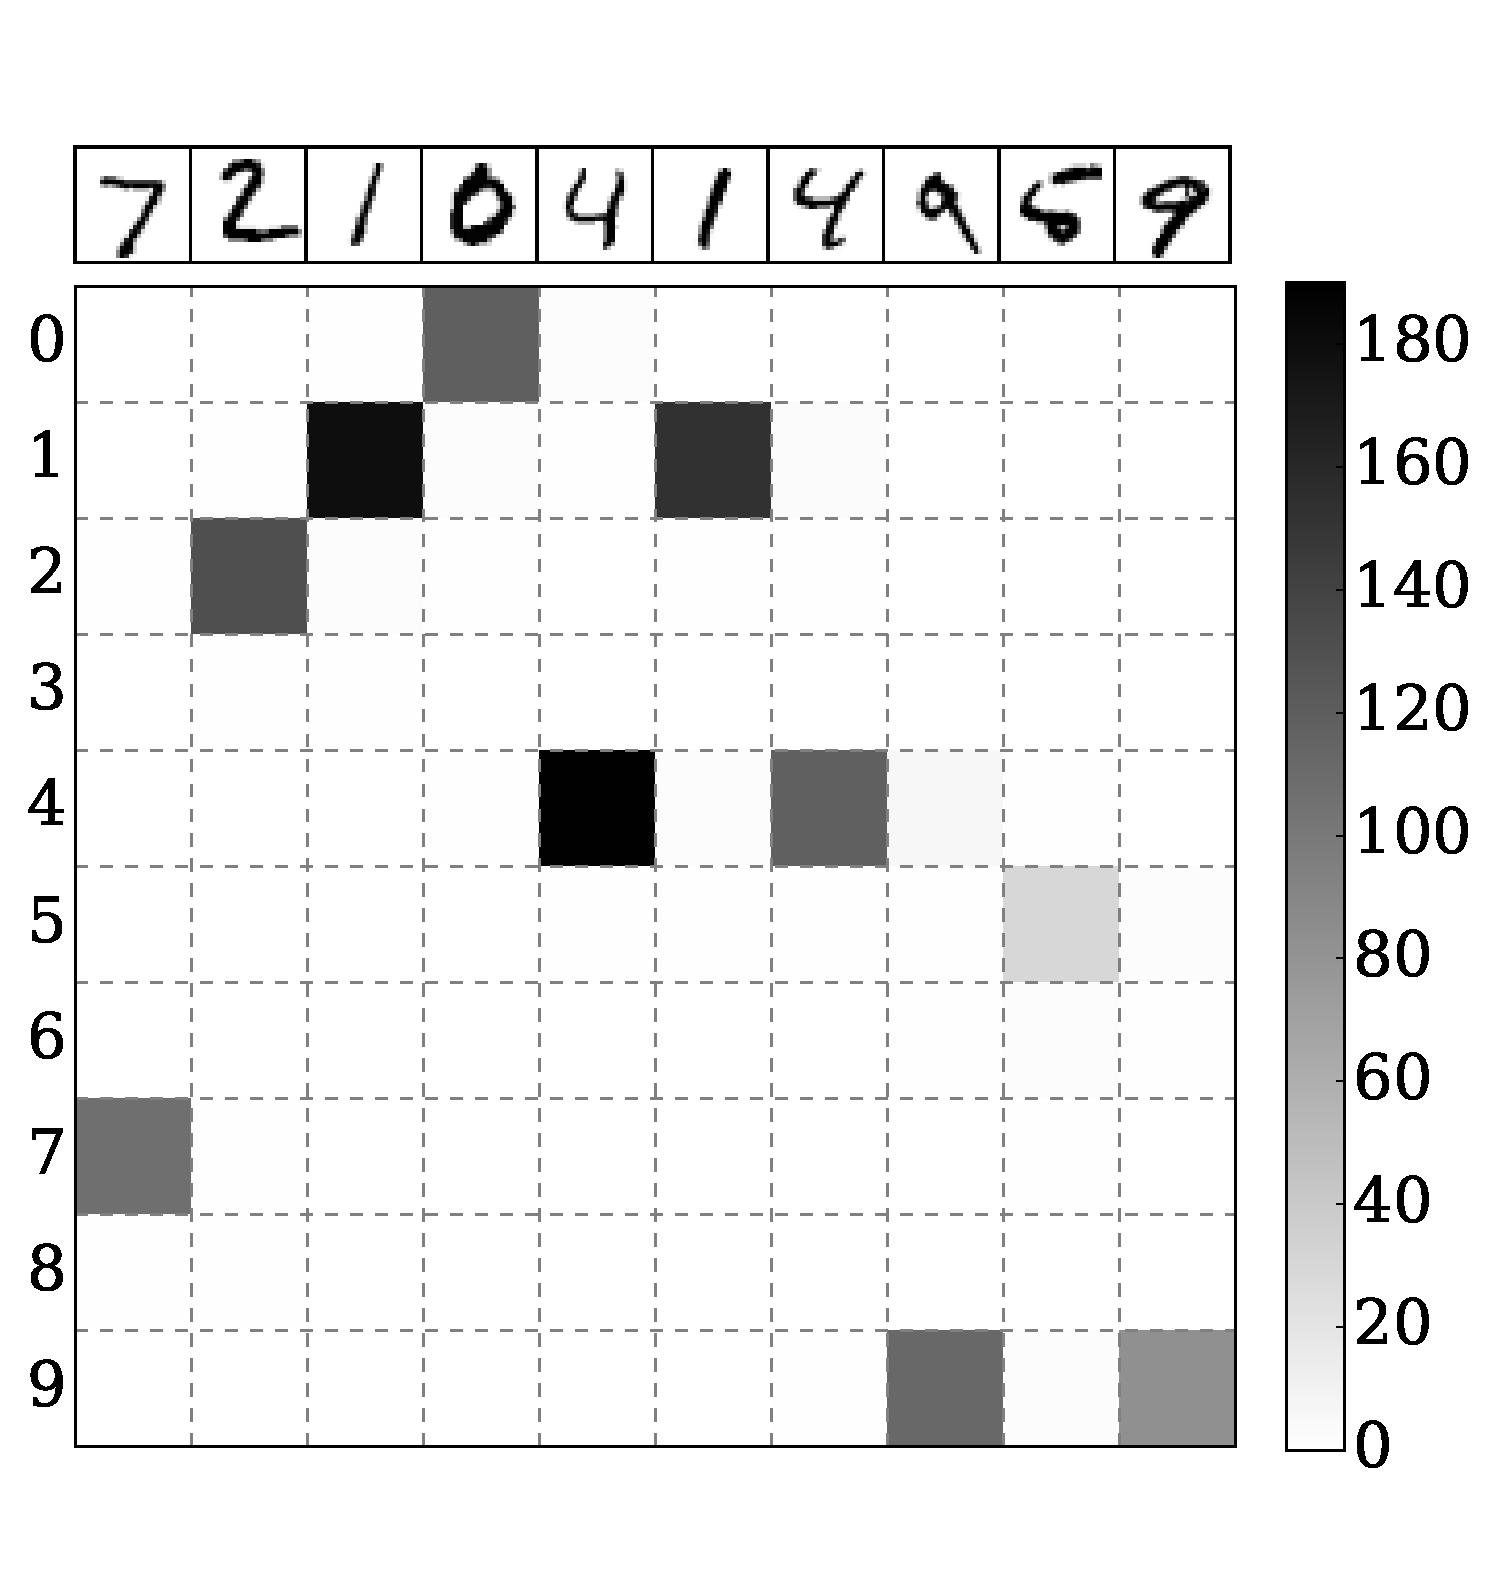
\includegraphics[width=\textwidth]{pics_iconip/7.pdf}
			\caption{Output firing rates of classification neurons.}
		\end{subfigure}
		\caption{Images presented in spike trains convolve with a weight kernel. (a) The $28\times28$ Poisson spike trains in raster plot, representing 10 digits in MNIST. (b) The firing rate of all the 784 neurons of the fourth image, digit `0', is plotted as a 2D image.
		(c) One out of six of the trained kernels ($5\times5$ size) in the first convolutional layer.
		(d) The spike trains plotted as firing rate of the neurons in the convolved 2D map.
		(e) Output firing rates for recognising these digits.}
		\label{fig:cnn}
	\end{figure}

%	Figure~\ref{fig:cnn} shows the small test of ten MNIST digits presented in Poisson spike trains for 1~s each.
%	A trained $5\times5$ kernel (Figure~\ref{fig:cnn}(c)) was convolved with these input digits, and the fourth digit `0' (Figure~\ref{fig:cnn}(b)) and its convolved output of the feature map was shown in Figure~\ref{fig:cnn}(d) as firing rate.
%	The output firing rate was recorded during a real-time SNN simulation on NEST, and compared to the modelled activations of Equation~\ref{equ:full_act} in ANNs.
%	
%	The input $x$ of the network was calculated as Equation~\ref{equ:mi_input}: $x_i=\lambda_i\tau_{syn}$, and so as the weighted sum of the synaptic current (see Equation~\ref{equ:mi_input}), $net_j$ and its variance (see Equation~\ref{equ:si_input}), $\sigma^2_j$.
%	With three combined activation functions as Equation~\ref{equ:full_act}:
%	\begin{equation}
%	\begin{aligned}
%	&\textrm{(1) Noisy Softplus:~~}  y_j=k \sigma_j \log [1 + \exp(\frac{net_j}{k \sigma_j})] \times S \times \tau_{syn}~~,  \\
%	&\textrm{(2) ReLU:~~ } y_j=max(0, net_j) \times S \times \tau_{syn}~~, \\
%	&\textrm{(3) Softplus:~~ } y_j=k \sigma \log [1 + \exp(\frac{net_j}{k \sigma})] \times S \times \tau_{syn}~~, ~~~\sigma=0.45,  
% 	\end{aligned}
%	\end{equation}	
%	we compare the output to the recorded SNN simulations.
%	ReLU assumes a non-noise current, and Softplus takes a static noise level thus $\sigma_j$ is not used for either of them, meanwhile Noisy Softplus adapts to noise automatically with $\sigma_j$.
%	The experiment took the sequence of 10 digits shown in Figure~\ref{fig:cnn}(a) to the same kernel and the estimated spike counts using Noisy Softplus fit to the real recorded firing rate much more accurately than ReLU and Softplus,  see~\ref{fig:af_compare}.
%%	Figure~\ref{fig:af_stast} illustrated the statistics of error between the estimation and the recorded firing rate, $err = y_j - \lambda_j$ which formed normal distributions where Noisy Softplus hold the weakest mean (low in abstract) and lowest standard deviation.
%	The Euclidean distance, $\sqrt{\sum_{j}(y_j/\tau_{syn} - \lambda_j)}$, between the spike counts and the predicted firing rates by Noisy Softplus, ReLU and Softplus was 184.57, 361.64 and 1102.76 respectively.
%	We manually selected a static noise level of 0.45 for Softplus, whose estimated firing rates located roughly on the top slope of the real response activity.
%	This resulted in longer Euclidean distance than using ReLU, since most of the input noisy currents were of relatively low noise level in this experiment.
%	Hence, the firing rate driven by lower noise level is closer to ReLU curve than Softplus.
	
	The estimated spike counts using NSP fitted the real recorded firing rate much more accurately than ReLU and Softplus.
	%	Figure~\ref{fig:af_stast} illustrated the statistics of error between the estimation and the recorded firing rate, $err = y_j - \lambda_j$ which formed normal distributions where NSP hold the weakest mean (low in abstract) and lowest standard deviation.
	The Euclidean distances, $\sqrt{\sum_{j}(\lambda_j' - \lambda_j)^2}$, between the spike counts and the predicted firing rates by NSP, ReLU and Softplus were 184.57, 361.64 and 1102.76 respectively.
	We manually selected a static noise level of 0.45 for Softplus, whose estimated firing rates located roughly on the top slope of the real response activity.
	This resulted in a longer Euclidean distance than using ReLU, since most of the input noisy currents were of relatively low noise level in this experiment.
	Hence, the firing rate driven by the lower noise level is closer to ReLU curve than Softplus.
			
	\begin{figure}[tbh!]
		\centering
		\begin{subfigure}[t]{0.48\textwidth}
			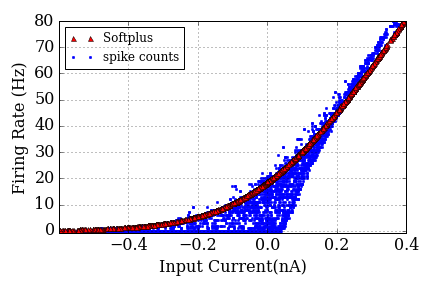
\includegraphics[width=\textwidth]{pics_iconip/6-5-1.png}
		\end{subfigure}
		\begin{subfigure}[t]{0.48\textwidth}
			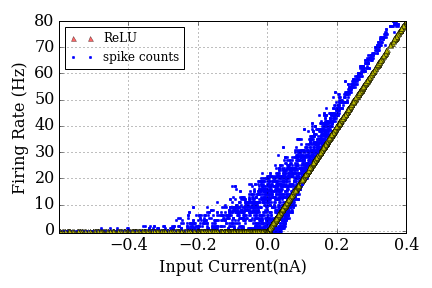
\includegraphics[width=\textwidth]{pics_iconip/6-5-2.png}
		\end{subfigure}\\
		\begin{subfigure}[t]{0.6\textwidth}
			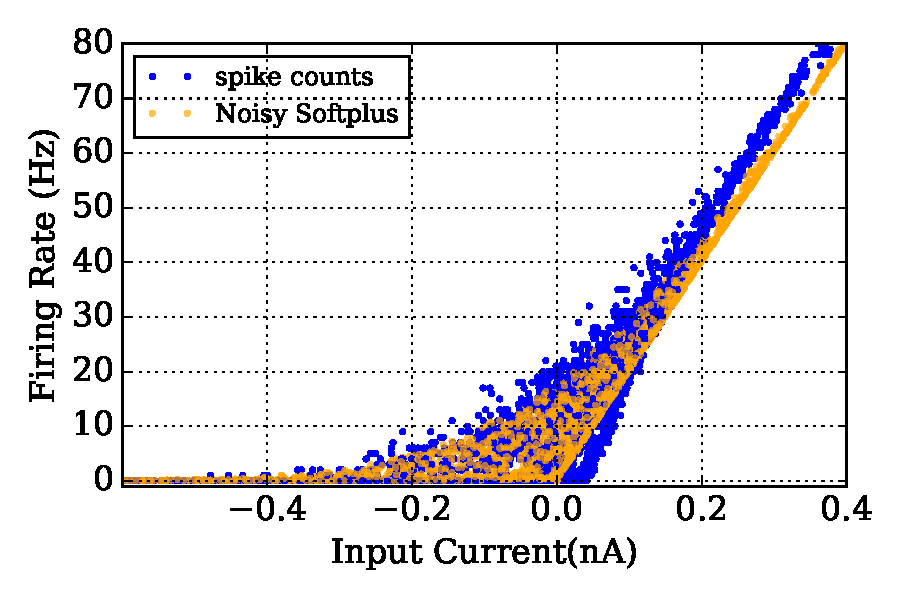
\includegraphics[width=\textwidth]{pics_iconip/6-5-3.pdf}
		\end{subfigure}
		\caption{
			The recorded firing rate of the convolution of the same kernel with 10 images in SNN simulation, compared to the firing rate prediction by $S \times f(x)$.
			NSP (a) fits to the neural response firing rate of LIF neurons more closely than ReLU (b) and Softplus (c).}
		\label{fig:af_compare}
	\end{figure}
	
	Figure~\ref{fig:cnn}(e) demonstrates the output firing rates of the 10 recognition neurons when tested with the digit sequence.
	The SNN successfully classified the digits where the correct label neuron fired the most.
	We trained the network with binary labels on the output layer, thus the expected firing rate of correct classification was $1/\tau_{syn}=200$~Hz according to Equation~\ref{Fig:tneuron}.
	The firing rates of the recognition test fell to the valid range around 0 to 200~Hz.
%	This shows another advantage of the proposed ANN-trained method that we can constrain the expected firing rate of the top layer, thus preventing SNN from exceeding its maximum firing rate, for example 1000~Hz when time resolution of SNN simulation set to 1~ms.
%		\begin{figure}[tbp!]
%			\centering
%			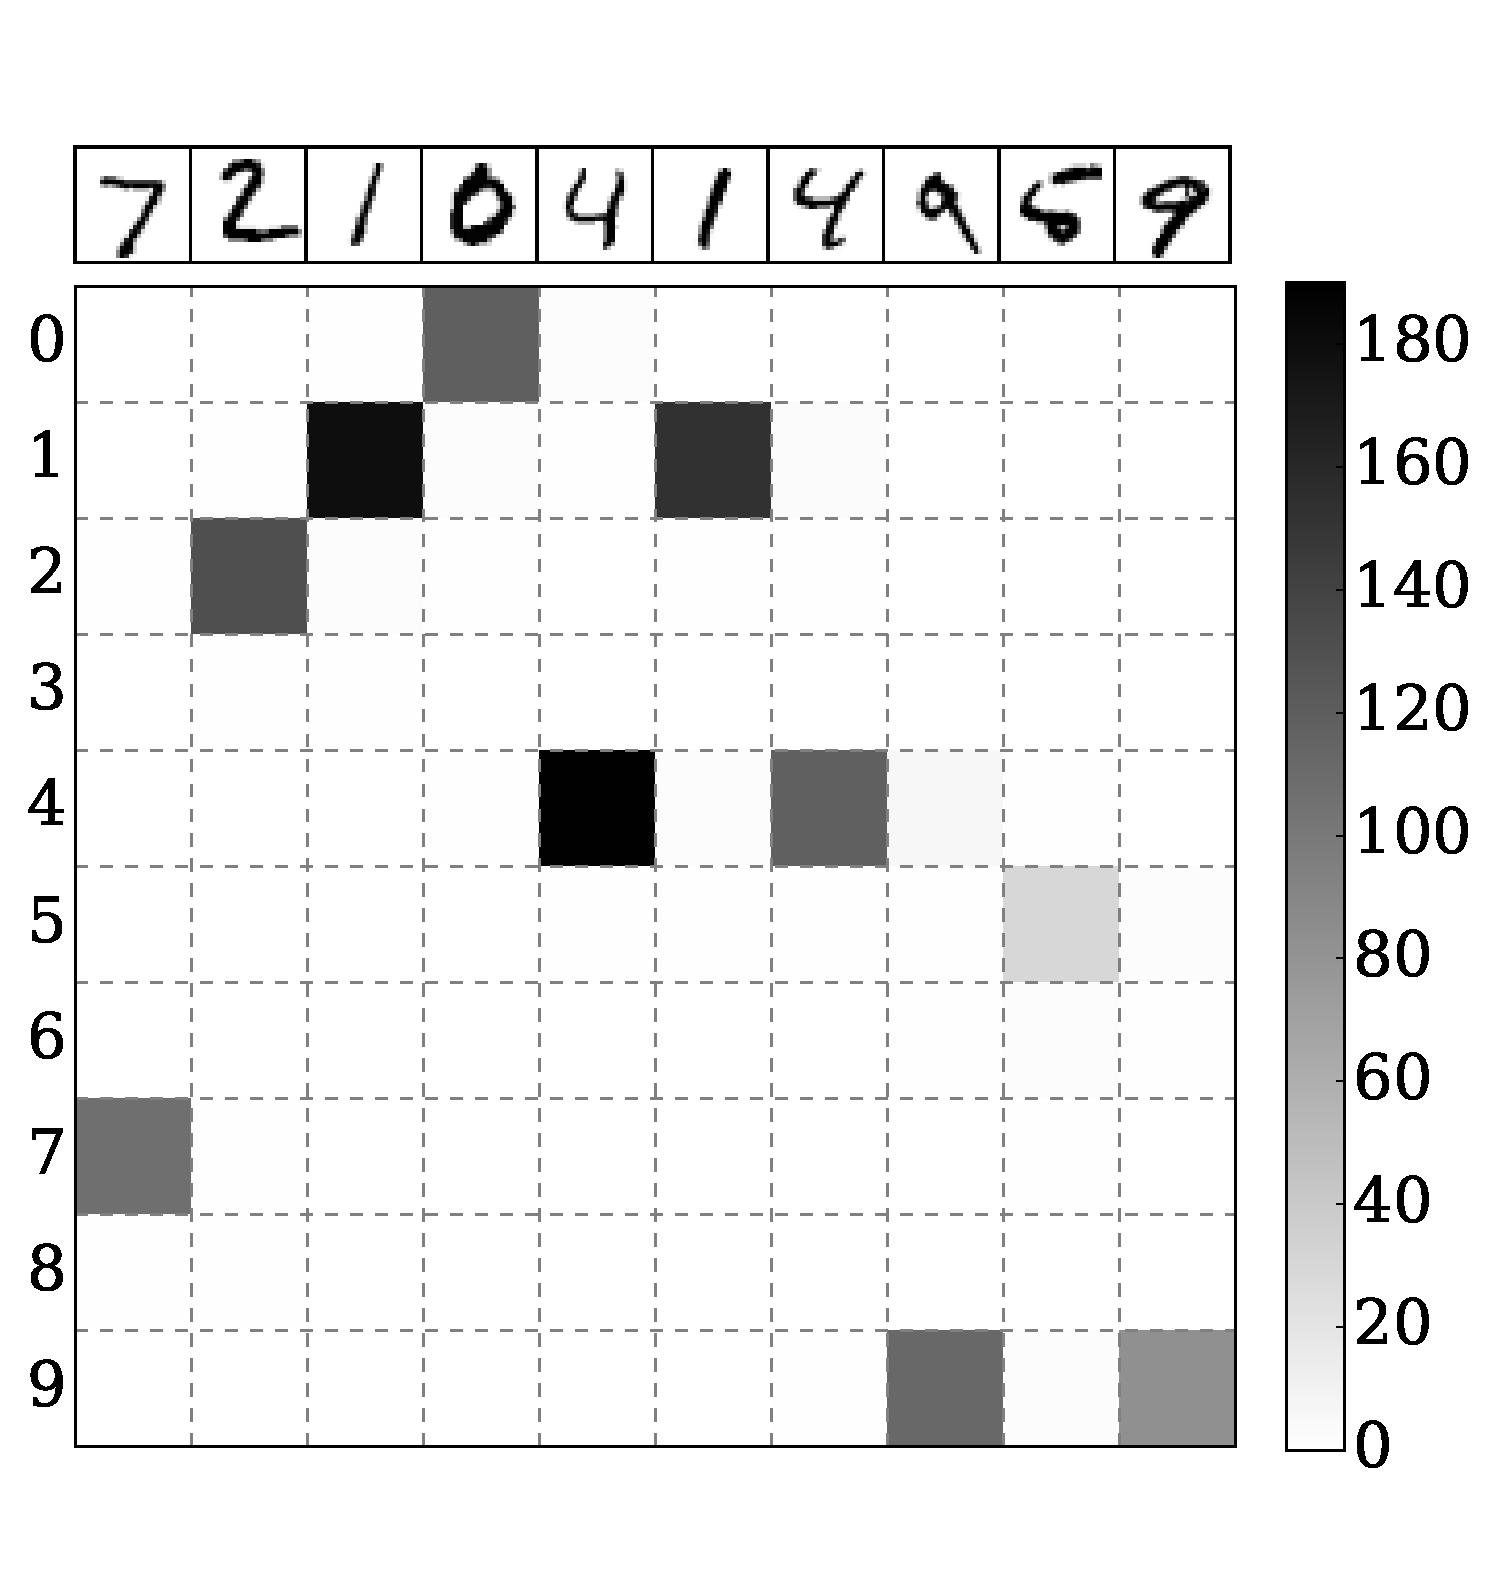
\includegraphics[width=0.6\textwidth]{pics_iconip/7.pdf}
%			\caption{Output firing rates for recognising 10 hand written digits.}
%			\label{Fig:out}
%		\end{figure}
	This shows another advantage of the NSP that we can estimate the firing rate of an SNN by $S \times f_{\textit{\textrm{NSP}}}(x)$ running its equivalent ANN, instead of simulating SNNs.
	Moreover, we can constrain the expected firing rate of the top layer, thus preventing the SNN from exceeding its maximum firing rate, for example 1~KHz when the time resolution of the simulation is set to 1~ms.
	
	\subsection{Learning Performance}
	\label{subsec:result_compare}
%	Here we focus on the recognition performance of the proposed ANN-trained SNN method.
%	Before looking into the recognition results, it is significant to see the learning capability of the proposed activation function, Noisy Softplus.
%	We compared the training using ReLU, Softplus, and Noisy Softplus by their loss during training averaged over 3 trials, see Figure~\ref{Fig:loss_ns}.
%	ReLU learned fastest with the lowest loss, thanks to its steepest derivative.
%	In comparison, Softplus accumulated spontaneous firing rates layer by layer and its derivative may experience vanishing gradients during back propagation, which result in a more difficult training.
%	Noisy Softplus performance lay between these two in terms of loss and learning speed.
%	However, the loss stabilised fastest, which means a possible shorter training time.
	Before looking into the recognition results, it is significant to see the learning capability of the novel activation function, NSP.
	We compared the training using ReLU, Softplus, and NSP by their loss during training averaged over three trials, see Figure~\ref{Fig:loss_ns}.
	ReLU learned fastest with the lowest loss, thanks to its steepest derivative.
	In comparison, Softplus accumulated spontaneous `firing rates' layer-by-layer and its derivative may experience gradual or even vanishing gradients during back propagation, which result in a more difficult training.
	The performance of NSP lied between these two in terms of loss and learning speed.
	The loss stabilised to the same level of the Softplus', because of the same problem of gradual gradients.
	However, it stabilised faster thanks to the accurate modelling of the noise, which means a possibly shorter training time.
	\begin{figure}[tbp!]
		\centering
		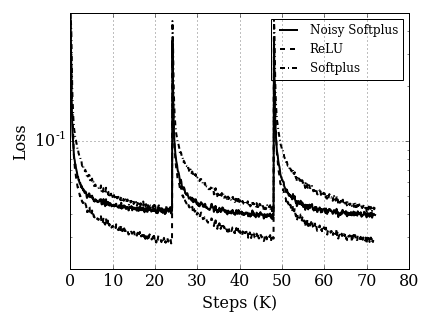
\includegraphics[width=0.7\textwidth]{pics_iconip/8.png}
		\caption{Comparisons of Loss during training using Noisy Softplus, ReLU and Softplus activation functions. Bold lines show the average of three training trials, and the grey colour illustrates the range between the minimum and the maximum values of the trials.  }
		\label{Fig:loss_ns}
	\end{figure}
%	The trained networks were scaled to SNNs and compared on recognition rates, 93.34\%, 96.43\% and 97.03\% with a conversion loss of 4.76\%, 0.91\% and 0.74\%.

\subsection{Recognition Performance}	
	\begin{figure}[tbp!]
		\centering
		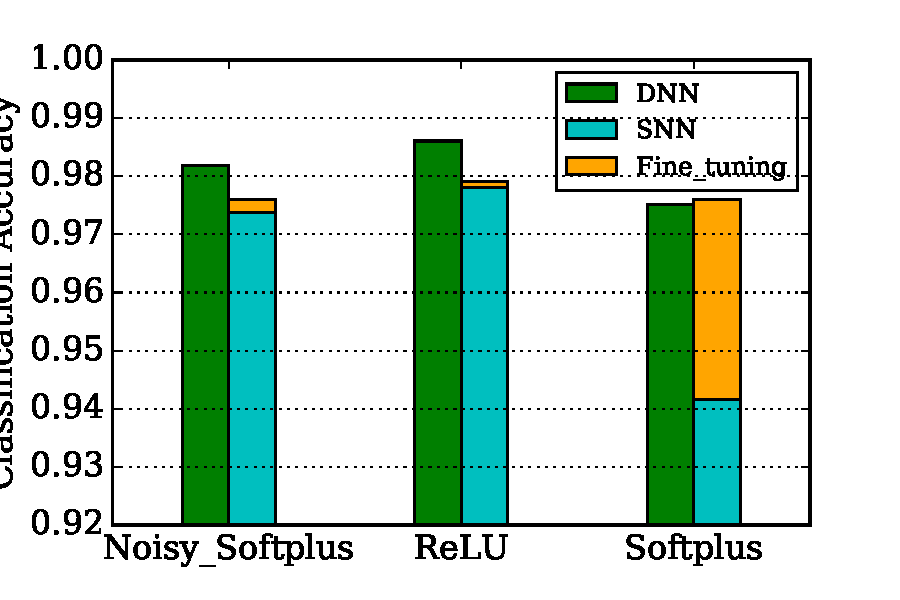
\includegraphics[width=0.7\textwidth]{pics_iconip/9-2.pdf}
		\caption{Classification accuracy.
			The trained weights were tested using the same activation function as training (DNN\_Orig), then transferred to SNN and tested on NEST simulation (SNN\_Orig), and finally fine-tuned to be tested on SNN (SNN\_FT) as well.  }
		\label{Fig:result_bar}
	\end{figure}
	The classification errors for the tests are investigated by comparing the average classification accuracy among three trials, shown in Figure~\ref{Fig:result_bar}.
	At first, all trained models were tested on the same artificial neurons as used for training in ANNs, and these experiments were called the `DNN' test since the network had a deep structure (6 layers).
	Subsequently, the trained weights were directly applied to the SNN without any transformation, and these `SNN' experiments tested their recognition performance on the NEST simulator.
	From DNN to SNN, the classification accuracy declines by 0.80\%, 0.79\% and 3.12\% on average for NSP, ReLU and Softplus.
	The accuracy loss was caused by the mismatch between the activations and the practical response firing rates, see examples in Figure~\ref{fig:af_compare}, and the strict binary labels for NSP and Softplus activations.
	Fortunately, the problem is alleviated by fine tuning which increased the classification accuracy by 0.38\%, 0.19\% and 2.06\%, and resulted in the total loss of 0.43\%, 0.61\%, and 1.06\% respectively.
	%	The order of total losses of these activation functions followed the Euclidean distance measured in Section~\ref{subsec:activity}.
	Softplus benefits the most from fine tuning, since the huge mismatch~(Figure~\ref{fig:af_compare}(c)) of response firing rate is greatly corrected.
	The improvement of NSP was obtained from the offset on the labels which helps the network to fit practical SNNs.
	As the recognition performance of ReLU is already high, there's little room for improvement.
	Even though the fine-tuning procedure does its job, the gain in accuracy is the smallest for this activation function.
	
	%	Thus fine tuning mainly corrects the mismatch between ReLU and the firing rates in SNNs, and constraints the output firing rates of the network.
	
	%	Thus fine tuning mainly corrects the mismatch between ReLU and the firing rates in SNNs, and constraints the output firing rates of the network.
	%	Softplus benefits the most from fine tuning, since not only the huge mismatch of response firing rate is greatly corrected, but also the offset on the labels helps the network to fit SNNs. 
	%dummy change
	
	%\begin{figure}[hbt!]
	%	\centering
	%	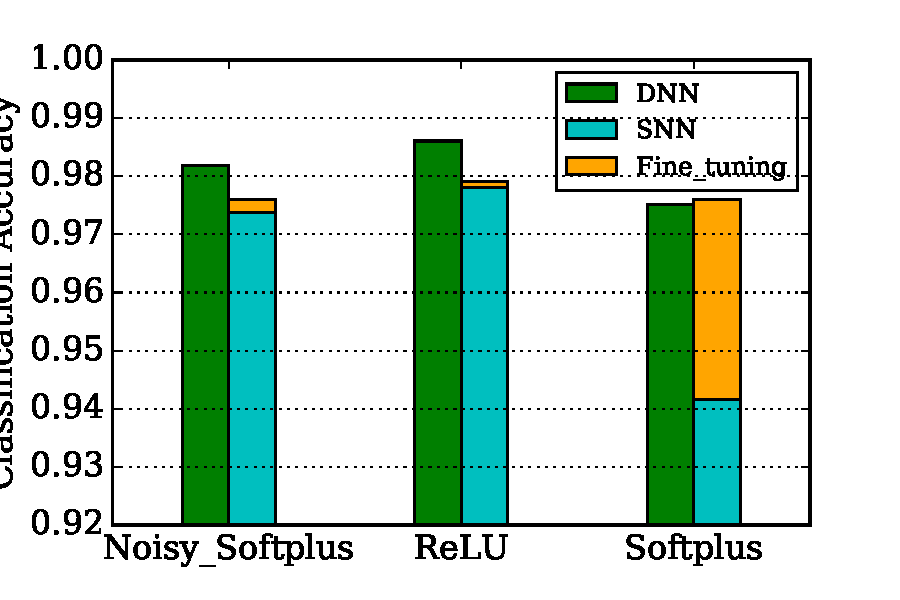
\includegraphics[width=0.7\textwidth]{pics_iconip/9-2.pdf}
	%	\caption{Classification accuracy compared among trained weights of NSP, ReLU, Softplus on DNN, SNN and fine-tuned SNN.}
	%	\label{Fig:result_bar1}
	%\end{figure}
	
	%\begin{table}[tbh] 
	%	\caption{Comparisons of classification accuracy (in \%) of ANN-trained convolutional neural models on original DNN, NEST simulated SNN, and SNN with fine-tuned (FT) model.}
	%	\begin{center}
	%		\bgroup
	%		\def\arraystretch{1.5}
	%		\begin{tabular} {r |c  c c |c c c |c c c}
	%			%First line
	%			\hline
	%			Trial No.
	%			&\multicolumn{3}{c|}{1} 
	%			&\multicolumn{3}{c|}{2}
	%			&\multicolumn{3}{c}{3}\\
	%			\hline
	%			Model
	%			& DNN & SNN &FT
	%			& DNN & SNN &FT
	%			& DNN & SNN &FT\\
	%			\hline
	%			\textbf{Noisy Sofplus}
	%			& 1.91 & 2.76 &2.45
	%			& 1.79 & 2.56 &2.19
	%			& 1.76 & 2.55 &2.10\\
	%			%				& 98.09 & 97.24 &97.55
	%			%				& 98.21 & 97.44 &97.81
	%			%				& 98.24 & 97.45 &97.90\\
	%			%				\hline
	%			\textbf{ReLU}
	%			& 1.36 & 2.03 &1.88
	%			& 1.46 & 2.28 &2.00
	%			& 1.36 & 2.25 &2.12\\
	%			%				& 98.64 & 97.97 &98.12
	%			%				& 98.54 & 97.72 &98.00
	%			%				& 98.64 & 97.75 &97.88\\
	%			%				\hline
	%			\textbf{Sofplus}
	%			& 2.30 & 5.66 &3.91
	%			& 2.75 & 5.22 &3.55
	%			& 2.42 & 6.62 &3.87\\
	%			%				& 97.70 & 94.34 &96.09
	%			%				& 97.25 & 94.78 &96.45
	%			%				& 97.58 & 93.38 &96.13\\
	%			\hline
	%		\end{tabular}
	%		\egroup
	%		\label{tbl:ns_result}
	%	\end{center}
	%\end{table}
	
	
	
	
	%	The best classification accuracy achieved by SNNs was trained with ReLU and fine-tuned by NSP.
	The most efficient training in terms of both classification accuracy and algorithm complexity, takes PAF-ReLU for ANN training and PAF-NSP for fine tuning.
	%	Softplus does not exhibit better classification capability and, more importantly, the manually selected static noise level hugely influences the mismatch between the predicted firing rates and the real data.
	%	Although NSP shows the least classification drop from ANNs to SNNs, the training performance is still worse than ReLU.
	%	Improved back propagation or other learning algorithms using noise level will be listed in the future work. 
	The best classification accuracy achieved by a larger spiking ConvNet~(784-16c-16p-64c-64c-10fc) was 99.07\% after fine tuning, a 0.14\% drop from the ANN test (99.21\%).
	The network reached the recognition rate of 98.7\% even without fine tuning, thus we suggest to make fine tuning an optional step for training.
	%	which was trained with PAF-ReLU and fine-tuned using PAF-NSP.
	
	
	It is useful to compare with existing SNN training methods shown in Table~\ref{tbl:compare_paf} where we order them on the computation complexity (descending).
	%	The generalised training method this paper proposed wins the other methods over the simplest activation function, and no conversions are requited of trained weights to be transferred to SNNs, they are well fitted to biologically-plausible LIF neurons, and only an optional additive processing of fine tuning.
	The generalised training method presented in this paper has a simple activation function, it requires no conversions of trained weights, which are well fitted to biologically-plausible LIF neurons, and has a single \emph{optional} additional processing of fine tuning.
	The combination of these features compose a method with exceptional performance and ease of use for training SNNs.
	
	
	\begin{sidewaystable*}[htbp] \small
		\caption{SNN training methods comparison.}
		\begin{center}
			\bgroup
			\def\arraystretch{1.1}
			\begin{tabular}{l c c c c c c}
				\cline{1-6}
				\begin{mycell}{3cm} Method \end{mycell} & 
				%  					\begin{mycell}{1.8cm} Computation\\Complexity \end{mycell} & 
				\begin{mycell}{1.8cm}Activation\\Function\end{mycell} &
				\begin{mycell}{1.8cm} Biologically-\\plausibility \end{mycell} &  
				\begin{mycell}{1.8cm} Additional\\Processing \end{mycell} &
				\begin{mycell}{1.8cm} Conversion \end{mycell} & 
				\begin{mycell}{3cm} Classification\\Accuracy(\%) \end{mycell} 
				\\
				\hline
				\begin{mycell}{3cm} \cite{Jug_etal_2012} \end{mycell} & 
				%  					\begin{mycell}{1.8cm} 1st \end{mycell} & 
				\begin{mycell}{1.8cm}Siegert \end{mycell} &
				\begin{mycell}{1.8cm} \textbf{Yes} \end{mycell} &  
				\begin{mycell}{1.8cm} \textbf{No} \end{mycell} & 
				\begin{mycell}{1.8cm} \textbf{No} \end{mycell} & 
				\begin{mycell}{3cm} 94.94\\~\cite{Stromatias2015scalable} \end{mycell} 
				\\
				\begin{mycell}{3cm} \cite{hunsberger2015spiking} \end{mycell} & 
				%  					\begin{mycell}{1.8cm} 2nd \end{mycell} & 
				\begin{mycell}{1.8cm} Soft LIF \end{mycell} &
				\begin{mycell}{1.8cm} \textbf{Yes} \end{mycell} &  
				\begin{mycell}{2.2cm} Noisy inputs\\ \&Activations \end{mycell} & 
				\begin{mycell}{1.8cm} \textbf{No} \end{mycell} & 
				\begin{mycell}{3cm} 98.37 \end{mycell}
				\\
				\begin{mycell}{3cm} \cite{diehl2015fast} \end{mycell} & 
				%  					\begin{mycell}{1.8cm} 3rd \end{mycell} & 
				\begin{mycell}{1.8cm} \textbf{ReLU} \end{mycell} &
				\begin{mycell}{1.8cm} No \end{mycell} &  
				\begin{mycell}{1.8cm} Dropout  \end{mycell} & %\&\\Conversion
				\begin{mycell}{1.8cm} Yes \end{mycell} &  
				\begin{mycell}{3cm} \textbf{99.1} \end{mycell} 
				\\
				\begin{mycell}{3cm} This\\Paper \end{mycell} & 
				%  					\begin{mycell}{1.8cm} 3rd \end{mycell} & 
				\begin{mycell}{1.8cm} \textbf{PAF}\\($p\times$ReLU)\end{mycell} &
				\begin{mycell}{1.8cm} \textbf{Yes} \end{mycell} &  
				\begin{mycell}{2.2cm} \textbf{No} \\or fine tune  \end{mycell} & 
				\begin{mycell}{1.8cm} \textbf{No} \end{mycell} & 
				\begin{mycell}{3cm} 98.72\\ \textbf{99.07(fine tune)} \end{mycell}  
				\\
				\cline{1-6}
				% contents!
			\end{tabular}
			\egroup
		\end{center}
		\label{tbl:compare_paf}
\end{sidewaystable*}
	
	%The network structure was the same with the state-of-the-art model which reported the best classification accuracy of 99.1\%~\cite{diehl2015fast} in ANN-trained SNNs: 12c5-2s-64c5-2s-10fc.
	%Their nearly loss-less conversion from ANNs to SNNs was achieved by using IF neurons, while our network performs the best among SNNs consisted of LIF neurons to our knowledge.
	
	\begin{figure}[htb!]
		\centering
		\begin{subfigure}[t]{0.49\textwidth}
			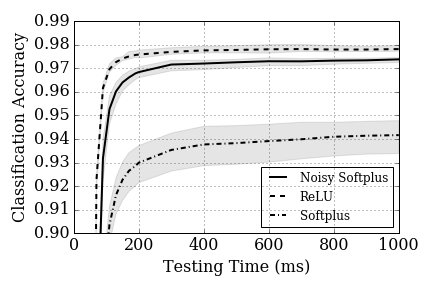
\includegraphics[width=\textwidth]{pics_iconip/8-2.png}
			\caption{Before fine tuning}
		\end{subfigure}
		\begin{subfigure}[t]{0.49\textwidth}
			\includegraphics[width=\textwidth]{pics_iconip/8-3.png}
			\caption{After fine tuning.}
		\end{subfigure}
		
		\caption{The classification accuracy of 3 trials (averaged in bold lines, grey shading shows the range between minimum to maximum) over short response times, with (a) trained weights before fine tuning, and (b) after fine tuning.}
		\label{fig:ca_time}	
	\end{figure}
	
	As it is a major concern in neuromorphic vision, the recognition performance over short response times is also estimated in Figure~\ref{fig:ca_time}.
	After fine tuning, Softplus significantly reduced the mismatch since the randomness among the three trials shrinks to a range similar to other experiments.
	Fine tuning also improved its classification accuracy and the response latency.
	Notice that all of the networks trained by three different activation functions showed a very similar stabilisation curve, which means they all reached an accuracy close to their best after only 300~ms of biological time. 
	
	
	\subsection{Power Consumption}
	Noisy Softplus can easily be used for energy cost estimation for SNNs.
	For a single neuron, the energy consumption of the synaptic events it triggers is:
	\begin{equation}
	\begin{aligned}
	E_{j} &= \lambda_j N_j T E_{syn}\\
	&= \dfrac{y_j N_j T E_{syn}}{\tau_{syn}}~~,
	\end{aligned}
	\label{equ:energy}
	\end{equation}
	where $\lambda_j$ is the output firing rate, $N_j$ is the number of post-synaptic neurons it connects to, $T$ is the testing time, and $E_{syn}$ is the energy cost for a synaptic event of some specific neuromorphic hardware, for example, about 8~nJ on SpiNNaker~\cite{stromatias2013power}.
	Thus to estimate the whole network, we can sum up all the synaptic events of all the neurons:
	\begin{equation}
	\sum_j E_{j} =  \dfrac{T E_{syn}}{\tau_{syn}} \sum_{j}y_j N_j.
	\end{equation}
	Thus, it may cost SpiNNaker 0.064~W, 192~J running for $3,000$~s with synaptic events of $8\times10^6/s$ to classify $10,000$ images (300~ms each) with an accuracy of 98.02\%.
	The best performance reported using the larger network may cost SpiNNaker 0.43~W operating synaptic event rate at $5.34\times10^7/s$, consume 4271.6~J to classify all the images for 1~s each.

\section{Summary}
%\section{Discussions}
	We presented a generalised SNN training method to train an equivalent ANN and transfer the trained weights back to SNNs.
	This training procedure consists of two simple stages: first, estimate parameter $p$ for PAF using NSP, and second, use a PAF version of conventional activation functions for ANN training. % can be generalised to activation units other than NSP.
	%The training of a SNN model is exactly the same as ANN training, and 
	The trained weights can be directly used in SNN without any further transformation.
	This method requires the least computation complexity while performing most effectively among existing algorithms.
	% and even more straight-forward than the other ANN offline training methods which requires an extra step of converting ANN-trained weights to SNN's.
	
	In terms of classification/recognition accuracy, the performance of ANN-trained SNNs is nearly equivalent to ANNs, and the performance loss can be partially solved by fine tuning.
	The best classification accuracy of 99.07\% using LIF neurons in a PyNN simulation outperforms state-of-the-art SNN models of LIF neurons and is equivalent to the best result achieved using IF neurons~\cite{diehl2015fast}.
	An important feature of accurately modelling LIF neurons in ANNs is the acquisition of spiking neuron firing rates. These will aid deployment of SNNs in neuromorphic hardware by providing power and communication estimates, which would allow better usage or customisation of the platforms.